% warwickthesis.tex modified by M Hadley from utthesis.doc  Sept 96
% Significant changes were made in 2009, first to work seemlessly with pdflatex
% and secondly to use the setspace package to control linespacing -
% removing some incompatibilities that existed before.
% any comments or problems - contact me  <m.j.hadley@warwick.ac.uk>
%%%%%%%%%%%%%%%%%%%%%%%%%%%%%%%%%%%%%%%%%%%%%%%%%%%%%%%%%%%%%%%%%%%%%%%%%%%%%
%%%
%%% File: utthesis.doc, version 2.0, January 1995
%%% =============================================
%%% Copyright (c) 1995 by Dinesh Das.  All rights reserved.
%%% This file is free and can be modified or distributed as long as
%%% you meet the following conditions:
%%%
%%% (1) This copyright notice is kept intact on all modified copies.
%%% (2) If you modify this file, you MUST NOT use the original file name.
%%%
%%% This file contains a template that can be used with the package
%%% utthesis.sty and LaTeX2e to produce a thesis that meets the requirements
%%% of the Graduate School of The University of Texas at Austin.
%%%
%%% All of the commands defined by utthesis.sty have default values (see
%%% the file
%           warwickthesis.sty
%%%                        for these values).  Thus, theoretically, you
%%% don't need to define values for any of them; you can run this file
%%% through LaTeX2e and produce an acceptable thesis, without any text.
%%% However, you probably want to set at least some of the macros (like
%%% \thesisauthor).  In that case, replace "..." with appropriate values,
%%% and uncomment the line (by removing the leading %'s).
%%%
%%%%%%%%%%%%%%%%%%%%%%%%%%%%%%%%%%%%%%%%%%%%%%%%%%%%%%%%%%%%%%%%%%%%%%%%%%%%%
% all comments starting with %! have been added by M Hadley as
% part of the conversion for the university of warwick
%
%
%\documentclass[11pt,a4paper,twoside]{report}      %% LaTeX2e document.
%%* Removed twoside option which is no longer accepted - you might want to use it for drafts.
\documentclass[12pt,a4paper]{book}      %% LaTeX2e document.
\usepackage{warwickthesis,setspace,graphicx}     %!  setspace is used to control linepacing
\usepackage[square]{natbib}                    %! needed for Harvard style of references.
                                                %! for more notes see the bibliography section below
\usepackage{enumerate}  %! used for the library form, but you might find it useful too.
% \mastersthesis                     %% Uncomment one of these; if you don't
% \phdthesis                         %% use either, the default is \phdthesis.

%\thesisdraft                       %% Uncomment this if you want a draft
                                     %% version; this will print a timestamp
                                     %% on each page of your thesis.

 \leftchapter                       %% Uncomment one of these if you want
% \centerchapter                     %% left-justified, centered or
% \rightchapter                      %% right-justified chapter headings.
                                     %% Chapter headings includes the
                                     %% Contents, Acknowledgments, Lists
                                     %% of Tables and Figures and the Vita.
                                     %% The default is \centerchapter.

%\renewcommand{\familydefault}{cmss}  %! removed April 2009 because the default times font reads more easily
                                     %! for larger blocks of text.%!
                                     %! Added March 2003.
                                     %! This alternative is to use a sans serif font as in
                                     %!  the Warwick Corporate style.
                                     %! The default is Times, which is still acceptable.


\onehalfspacing                      %! This is the default and gives an acceptable "double spaced" thesis
                                     %! It is the minimum spacing accepted by the graduate school, and there is no reason to increase the spacing.
% \singlespacing                     %! Uncomment if you want single-spacing,
%\doublespacing                     %! uncomment if you want real double-spacing for some perverse reason.

%\setlength{\textheight}{9.0in}      %! Uncomment this for a slightly
                                     %! longer page. The default is now 8.5in (from Feb 2010)
                                     %! regulations require page numbers to be at least 1.5cm into the page.
                                     %! You can even try a longer page to save paper.

%! Double sided printing is no longer allowed (March 2008), it caused too many problems at binding,
                              %\setlength{\evensidemargin}{0.15in}  %! Uncomment this line for double sided printing
                                      %! Double-sided printing has recently been
                                      %! allowed by the Graduate School (March 2003)
                                      %! The default is {0.7in} for single sided.
%! Double sided printing is no longer allowed (March 2008), it caused too many problems at binding,

\renewcommand{\thesisdepartmentname}{Mathematics}    %! The name of
                                                  %   the department

%! \renewcommand{\thesissubmission}{Submitted to the University of Warwick\\
%!              in partial fulfilment of the requirements\\
%!                   for admission to the degree of\\}
%!
%!!!!!!!! default is:
%!
\renewcommand{\thesissubmission}{Submitted to the University of Warwick\\
                        for the degree of}
%!
%! In the title page this wording will be preceeded by:  thesis\\
%!                 and ended by:  Doctor of Philosophy   (or the
%!                                               selected alternative names
%! use \\ where you want a new line

\renewcommand{\thesisauthor} {Edwin Kutas}    %% Your official name.
\renewcommand{\thesisauthorno}{........}  %! your university number, used on the library copyright page.


\renewcommand{\thesismonth}{....}     %% Your month of graduation.

\renewcommand{\thesisyear}{....}      %% Your year of graduation.

\renewcommand{\thesistitle}{Log del Pezzo Surfaces, Degenerations and Torus Actions}     %% The title of your thesis; use
                                     %% mixed-case.

%! \renewcommand{\thesistitletypesize}{\LARGE}   %! Put this in if you
                                  %!   want a Large title the default is \large

\renewcommand{\thesisauthorpreviousdegrees}{....}
                                     %% Your previous degrees, abbreviated;
                                     %% separate multiple degrees by commas.

\renewcommand{\thesissupervisor}{Miles Reid}
                                     %% Your thesis supervisor; use mixed-case
                                     %% and don't use any titles or degrees.

\renewcommand{\thesisauthoraddress}{....}
                                     %% Your permanent address; use "\\" for
                                     %% linebreaks.
%%%%%%%%%%%%%%%%%%%%%%%%%%%%%%%%%%%


%%%%%%%%%%%%%%%%%%%%%%%%%%%%%%%%%%%%%%%%%%%%%%%%%%%%%%%%%%%%%%%%%%%%%%%%%%%%%
%%%
%%% The following commands are all optional, but useful if your requirements
%%% are different from the default values in utthesis.sty.  To use them,
%%% simply uncomment (remove the leading %) the line(s).

% \renewcommand{\thesisdegree}{...}  %% Uncomment this only if your thesis
                                     %% degree is NOT "DOCTOR OF PHILOSOPHY"
                                     %% for \phdthesis or "MASTER OF ARTS"
                                     %% for \mastersthesis.  Provide the
                                     %% correct FULL OFFICIAL name of
                                     %% the degree.

% \renewcommand{\thesisdegreeabbreviation}{...}
                                     %% Use this if you also use the above
                                     %% command; provide the OFFICIAL
                                     %% abbreviation of your thesis degree.

%\renewcommand{\thesistype}{Thesis}    %% Use this ONLY if your thesis type
                                     %! is NOT "Thesis"
                                     %% Provide the OFFICIAL type of the
                                     %% thesis; use mixed-case.

% \renewcommand{\thesistypist}{...}  %% Use this to specify the name of
                                     %% the thesis typist if it is anything
                                     %% other than "the author".

%%%
%%%%%%%%%%%%%%%%%%%%%%%%%%%%%%%%%%%%%%%%%%%%%%%%%%%%%%%%%%%%%%%%%%%%%%%%%%%%%


%\input header.tex          %! Input declarations, new
                              %theorems etc.


%%%%% - This horrific mess of packages needs to be cleaned

\usepackage{geometry}  
\geometry{letterpaper} 
\usepackage{graphicx}
%\usepackage[backend=bibtex]{biblatex}
\usepackage{array}
\usepackage{amssymb}
\usepackage{amsmath}
\usepackage{amsthm}
\usepackage{graphicx}
\usepackage[parfill]{parskip} 
\usepackage[utf8]{inputenc}
\usepackage[english]{babel}
\usepackage{tikz}
\usepackage{tikz-cd}
\usepackage[noend]{algpseudocode}
\usepackage{caption}
\usepackage{subcaption}
\usepackage{fancyhdr}
\usepackage{enumitem}
\usepackage[super]{nth}
\usepackage{comment}
\usepackage[colorlinks=true,linkcolor=blue]{hyperref}
\usepackage{blkarray} %This is for labelled matrices
\usetikzlibrary{decorations.pathreplacing} % this is for Ai's drawing
\usepackage{bbm}


%
%\pagestyle{fancy}
%\lhead{}
%\chead{}
%\rhead{}
%\lfoot{}
%\cfoot{\thepage}
%\rfoot{}
%\renewcommand{\headrulewidth}{0pt}
%\setlength{\footskip}{50pt}

%\makeatletter
%\def\BState{\State\hskip-\ALG@thistlm}
%\makeatother

\makeatletter
\def\thm@space@setup{%
  \thm@preskip= 10pt
  \thm@postskip=\thm@preskip % or whatever, if you don't want them to be equal
}
\makeatother


\newtheorem{thm}{Theorem}[section]
\newtheorem{cor}[thm]{Corollary}
\newtheorem{prop}[thm]{Proposition}
\newtheorem{lem}[thm]{Lemma}


\theoremstyle{definition}

\newtheorem{dfn}[thm]{Definition}
\newtheorem{ex}[thm]{Example}
\newtheorem{conj}[thm]{Conjecture}
\newtheorem*{rem}{Remark}
\newtheorem{assumption}[thm]{Assumption}
\newtheorem{algorithm}{Algorithm}



\newcommand{\Rom}[1]
    {\MakeUppercase{\romannumeral #1}}

\pgfdeclarelayer{edgelayer}
\pgfdeclarelayer{nodelayer}

\pgfsetlayers{edgelayer,nodelayer,main}

% Node styles
\tikzstyle{none} = []
\tikzstyle{Filled Basic}=[fill=black, draw=black, shape=circle]

% Edge styles
\tikzstyle{Dashed Line}=[-, draw=blue, dashed]
\tikzstyle{Filled Blue}=[-, draw=blue]
\tikzstyle{Dashed Black}=[-, draw=black, dashed]
\tikzstyle{Red}=[-, draw={rgb,255: red,191; green,0; blue,64}]
\tikzstyle{new edge style 0}=[-, dashed, draw={rgb,255: red,191; green,0; blue,64}]

\tikzstyle{Dashed Line}=[-, draw=blue, dashed]
\tikzstyle{none} = []
\tikzstyle{new edge style 1}=[<->, thick]
\tikzstyle{new edge style 2}=[{<- left hook}]

\graphicspath{ {images/} }


\newcommand{\N}{\mathbb{N}}
\newcommand{\C}[1]{(\mathbb{C}^*)^#1}
\newcommand{\ldp}{log del Pezzo}
\newcommand{\mb}[1]{\mathbb{#1}}
\newcommand{\Hi}{Hirzebruch surface }
\newcommand{\minres}{minimal resolution}
\newcommand{\LJ}{Looijenga pair}
\newcommand{\ra}{\rightarrow}
\newcommand{\spl}{\text{SL}_2 (\mathbb{C})}
\newcommand{\gl}{\text{GL}_2 (\mathbb{C})}
\newcommand{\pgl}{\text{PGL}_2 (\mathbb{C})}
\newcommand{\wt}[1]{\widetilde #1}
\newcommand{\Q}{\mathrm{Q}}
\newcommand{\Z}{\mathrm{Z}}
\newcommand{\F}{\mathrm{F}}
\renewcommand{\P}{\mathrm{P}}



\begin{document}



%%* Uncomment a ttitle page.
%%% 2018 only colour is available now. Use printer settings for black and white
%%%  \thesistitlepage                     %% Generate the title page.
\thesistitlecolourpage           %! Generates a COLOUR title page.

%%* Start roman page numbering here for contents, etc
\pagenumbering{roman} %! Begins roman numerals start from page i.

\tableofcontents                     %% Generate table of contents.
% \listoftables                      %% Uncomment this to generate list
                                     %% of tables.
% \listoffigures                     %% Uncomment this to generate list
                                     %% of figures.

\begin{thesisacknowledgments}        %% Use this to write your
%  \input ack.tex                    %% acknowledgments; it can be anything
                                     %% allowed in LaTeX2e par-mode.

                                     %! This following is not needed, but you may like to add it.
%This \lowercase\expandafter{\thesistype} was typeset with
%\LaTeXe\footnote{\LaTeXe{} is an extension of \LaTeX. \LaTeX{} is
%a collection of macros for \TeX. \TeX{} is a trademark of the
%American Mathematical Society. The style package {\em warwickthesis} was
%used.} by \thesistypist.

\end{thesisacknowledgments}

\begin{thesisdeclaration}        %! Use this to declare the extent of
                 %! the original work,
                 %! collaboration, other published
                                 %! material etc.it can be anything
                                 %% allowed in LaTeX2e par-mode.
Replace this text with a declaration of the extent of the original work,
collaboration, other published material etc. You can use any \LaTeX\
constructs.

\end{thesisdeclaration}


\begin{thesisabstract}               %% Use this to write your thesis
                                     %% abstract; it can be anything
                                     %% allowed in LaTeX2e par-mode.
%!  \begin{singlespace}       %! uncomment this if you need single spacing
%   \input abstract.tex       %!           don't forget the end spacing!
                                     %! It must fit on one page.
                                     %! single spacing and smaller
                                     %! font size
                                     %!  is allowed here.
%!   \end{singlespace}
\end{thesisabstract}

%\begin{thesisabbreviations}       %! Use this to give a list of
                                   %! abbreviateons
                                   %! It can be anything
%\end{thesisabbreviations}         %! allowed in LaTeX2e par-mode.
                                   %!The following may be useful':
                     %!\begin{itemize}
                     %!     \item[symbol]descriptive text..
                     %!\end{itemize}

%\end{thesisabbreviations}
%!!!!!!!!!!!!!!!                     %% Begin your thesis text here; follow
                                     %% the report style and group your text
                                     %% in chapters, sections, etc. eg:
%%* don't need this with one-sided printing
%\newpage{\pagestyle{empty}\cleardoublepage} %! ensure that Chapter 1 starts on an odd
                                           %! page when using double sided printing.
%%* Start arabic numbering of main text here
\pagenumbering{arabic} %! Begins arabic numerals start from page 1.


\chapter{Introduction}

% \input introduction.tex


                            %% More chapters.
%!
%! There are a few variations of reference

%!!!!!!!!!!!!!!!

%  \appendix                            %% this will do the appendices
%  \chapter{Proof of Fred's theorem}
%  \input{app1.tex}
%  \chapter{listing of Fred's program}
%  \input{app2.tex}

This thesis solves a range of classification problems for singular surfaces.


Throughout this thesis we consider varieties $X$ with $-K_X$ ample and various restrictions on the singularities. These are particular instances of Fano varieties. A two dimensional Fano variety is called a \ldp\ surface, see ~\ref{beginnersdef}. Smooth log del Pezzo surfaces were described in work in the late 19th century and early 20th century. These surface are all of the form $\mb{P}^2$ blown up in $k$ points where $k <9 $, or the exceptional case $\mb{P}^1 \times \mb{P}^1$. Such an elegant classification does not exist in the case of \ldp\ surfaces with singularities; as represented by \cite{CH}, \cite{MR2053462}. A lot of work has been done on extending this classification to singular surfaces. In particular recent approaches have been interested in using of machinery of toric degeneration's. This technique involves constructing a family $\mathcal{X}$ over $\mb{A}^1$ such that the fiber over $0$ is a normal surface that contains $\C{2}$ as a dense subvariety for which the natural action of the torus extends to the variety.  



 Work of \cite{CH} and \cite{AC} have established a one to one correspondence between \ldp\ surfaces with $h^0(-K_X) \neq 0$ and toric degenerations upto mutation subject to assumptions on the singularities of the surface. It has been conjectured that this one to one correspondence extends to other classes of singularities beyond those considered in the above papers. 
 
 
 
%We discuss these results in the following way:


In the case of surfaces it is interesting to study the log del Pezzos with log terminal singularities. In the full generality, a log terminal surface singularity is a group quotient by a subgroup of $\gl$. The case when the subgroup is cyclic is particularly important, and we refer to these as cyclic quotients. In the case of cyclic quotient singularities it has been conjectured that these admit toric degeneration.


This thesis is about log del Pezzo surfaces. The formal definition is:
\begin{dfn}\label{beginnersdef}
A log del Pezzo surface is a normal two dimensional variety over $\mb{C}$ which has only log terminal singularities and has $-K_X$ ample.
\end{dfn}
see Definition~\ref{Log terminal Singularity} for a definition of log terminal singularities.

Our motivating aim is the classification of such surfaces.
This is an absolutely hopeless task in full generality.
Nevertheless, we can classify special cases as follows.

\subsection{Log del Pezzo surfaces of complexity 1}
The Gorenstein index of a singularity $S$ is the smallest value $n$ such that $n K_S$ is Cartier. We define the Gorenstein index of a surface $X$ to be the smallest value $n$ such that $nK_X$ is Cartier.
For any given $i \in \mathbb{N}$, the set of deformation
families of log del Pezzo surfaces $X$ with Gorenstein index $i_X=i$
is finite \cite{f}.

It is worth noting that the number of families increases enormously as the Gorenstein
index of the surface increases. For example, only in the toric case, 
the start of the classification is
\[
\begin{tabular}{| c | c |}
\hline\\
\text{index $i$} & \text{number of toric surfaces}\\ \hline
1 & 16 \\
2 & 30 \\
3 & 99  \\
4 & 91  \\
5 & 250 \\
6 & 379 \\
7 & 429 \\
8 & 307 \\
9 & 690 \\
10 & 916 \\
\hline
\end{tabular}
\]

We consider these surfaces from three different and related points of view.

In particular, we classify log del Pezzo surfaces that admit a $\mathbb{C}^\times$ action.
In this thesis we give an algorithm to classify log del Pezzo surfaces that admit a $\mathbb{C}^\times$ action and which have only log terminal singularities. 


A normal variety $X$ of dimension $n$ equipped with an effective action of a torus of dimension $n-k$ is referred to as a variety of complexity $k$. To illustrate the notion, note first that a toric variety $X$ has an action of its $n$-dimensional `big torus' $T\subset X$, and equipped with this action $X$ is a variety of complexity~0.
One could also give consider $X$ equipped with the natural action of a $k$-dimensional
subtorus $T'\subset T$, and then $X$ is a variety of complexity~$k$. (See \S\ref{ToricDowngrade}.)

However, there are many varieties of complexity $k<n$ whose torus action does not extend to a toric variety. This is one of the main themes of this thesis: we study
and classify surfaces of complexity~1 that are not toric.

In this way, complexity provides a way of grading the difficulty of a classification problem. Significant progress has been made on this problem before: S\"{u}ss \cite{Suss} classifies log del Pezzo surfaces admitting a $\mathbb{C}^\times$ action which have picard rank one and Gorenstein index less than~3. Huggenberger \cite{Huggenberger} classifies log del Pezzo surfaces of complexity~1 that have index 1 and arbitrary picard rank. Ilten, Mishna and Trainor \cite{IMT} recover the same classification and extend it into higher dimension. The methods and language used are broadly the same (though, analogous to the language of toric geometry, it varies whether papers work in the lattice $N$ or its dual lattice $M$), though Huggenberger exploits Hausen's anticanonical complex technology to describe the Cox ring in detail. 

We extend these results by presenting an algorithm that classifies
log del Pezzo surfaces of complexity 1 with given index.
The algorithm works and \textbf{terminates for any} index, 
though since the index is an unbounded invariant, there is no hope of 
a closed-form classification via methods of this type for all such del Pezzo with a torus action.



\subsection{Bounded singularity content of log del Pezzo surfaces}

We can consider log del Pezzos from a completely different point of view. Rather than considering the global invariants, we can consider the local invariants of the singularities. 
It follows from the definition (Def \ref{}) that the singularities
are all finite quotient singularities, but this class of singularities itself is an infinite set. 
The {\em discrepancies} associated to a singularity (see Def~\ref{}) form a measure of
its complexity expressed as a collection of rational numbers, one for each curve in a resolution. 
When these numbers are small, but still greater than $-1$, the singularity may be regarded as `more complicated'. 
However surfaces that have only these more complicated singularities can be classified explicitly. Informally,
the basic reason is that it is hard to impose many of these singularities onto a single surface.

These conditions naturally arise as soon as you start to consider singularities in families. The first place this was considered was in \cite{CP} where they considered the case of $\frac{1}{p}(1,1)$ singularities, where $p \geq 5$. We extend this by


\begin{thm}[Theorem~\ref{ThmOnSing}]
Let $X$ be a surface with singularities of only small discrepancy then $X$ has at most one singularity except for one sporadic family. All of these log del Pezzo surfaces admit a toric degeneration.
\end{thm}

This reproves the results of \cite{CP} who classified log del Pezzo surfaces with only $\frac{1}{p}$ singularities and extends results in \cite{Cuzzo} who classified surfaces with $\frac{1}{5}(1,2)$  and $\frac{1}{p}(1,1)$ singularities.

We also consider how the cascade of these surfaces behaves. This notion was introduced in \cite{MR2053462} and is essentially asking for the birational relations between the surfaces. we prove that once our singularity is sufficiently complicated then you get a subset of the following series of birational relations

\[
\begin{tikzpicture}[baseline= (a).base]
\node[scale=.6] (a) at (0,0){
% https://tikzcd.yichuanshen.de/#N4Igdg9gJgpgziAXAbVABwnAlgFyxMJZABgBoBmAXVJADcBDAGwFcYkQANAAgF4uOA+sRABfUuky58hFAEYK1Ok1btBs0eJAZseAkQBMCmgxZtEIADoWAxlAg4EYiTulFyRpadUDg9ALQA1gKygQL6frIiGs5SeigALB4mKuaCvqEhQfpRTlqSujLI7vGKyWYgAJrReS5xyIYArKXK5RXBAHrqudqxhYlNxi3sbbLt+tU9BQakAGzNXuZWtHYOE-muCbPzKZYWy-aOmpMb9aQA7NutPmDBIp1rtX3nl8PXYXfj3et1DaSyL6kAOSAnz0YEZcFZcGRB69IgzUj6AGVYGwqYoBHEZEcYGgyHBfH6cHZNEnM6kLGDBa7WwHUl1AAcFOxuOEX0eRHJ-ypO2AI06IlR7LhKHJSJ55T5HWyQqO30KTO5nh2Vlpq2F6OQTPFyvKqpWhximoAnH9kVLgDdZFxgXdIsCuPTCqadWV2BabkTAR9BYCnURfgNdaoQb5ARDQkSIjk5RyMaQShLhn6NScEXMk6k8RGoX4Zf7RVtMzSDQWtUXg0ChGXyUG3eYpaN7TWE+b+fnU4zSHWhosbKXOwrW8X9XTB0RTYnKyAPWFvWNBWXTT3qbPZPPmyJFDAoABzeBEUAAMwAThAALZIeQgHAQJBkStgZiMRg0Rj0ABGMEYAAV5exGBgI8cGqU8LyQQwbzvRBr3rJ8XzfT9vz-OMQEA4DQLPS9EHcKCIMzeDXzQpDf3-cx0JA3IwOw3DbyQX5H2fIj3y-UjUIozDwMQRI8JwgimMQ1iUJFNCgMozRqPomg6MQBFGIQ4ihLI0SMKorCpN48l5OYkjhPRFTxOPdTZOk6CmW0wTkOUji1K4rSZNNCzFKs9ixM47DzJk2QHzggTnLYkSbIk4zHK82De0IyyAv0oKjK4nivOyYKuNkSCvPIWzsNS0yr3iTLcpymCGnyorCtkGYStkWjoNkM5Kuqq8GUqzzoP0YgSrawr9CSuKstC1rImSrL7Jq40SoS1qMqGiCGsQfQ8umubZv0YrFpWrqKrWuSZP0Oq1omiCmv2rqxrWlqkHIdq1v6i7Bt627CvIHqQEknCHxk8gMsoEQgA
\begin{tikzcd}
        &               &                  &                                     &                                                 &                                               & X''_{a''-k_1''-k_2''-2} \arrow[r] & \cdots \arrow[r]    & X''_0            &                   \\
        &               &                  &                                     &                                                 & X''_{a''-k_1''-k_2''-1} \arrow[rd] \arrow[ru] &                                   & {Y_1^1}'' \arrow[r] & \cdots \arrow[r] & {Y_{n_1 ''}^1}''  \\
        &               &                  &                                     &                                                 &                                               & Y'' \arrow[ru] \arrow[r]          & {Y_1^2}'' \arrow[r] & \cdots \arrow[r] & {Y_{n_2''}^2}''   \\
X = X_0 & X_1 \arrow[l] & \cdots \arrow[l] & X_{a-k_1-k_2-1} \arrow[l] \arrow[d] & X_{a-k_1-k_2} \arrow[l] \arrow[ruu] \arrow[rdd] &                                               &                                   &                     &                  &                   \\
        &               &                  & Y \arrow[ld] \arrow[rd]             &                                                 &                                               & Y' \arrow[rd] \arrow[r]           & {Y_1^2}' \arrow[r]  & \cdots \arrow[r] & {Y_{n_2'}^2}'     \\
        &               & Y_1^1 \arrow[d]  &                                     & Y_1^2 \arrow[d]                                 & X'_{a'-k_1'-k_2'-1} \arrow[ru] \arrow[rd]     &                                   & {Y_1^1}' \arrow[r]  & \cdots \arrow[r] & {Y_{n_1'}^1}'     \\
        &               & \vdots \arrow[d] &                                     & \vdots \arrow[d]                                &                                               & X_{a'-k_1'-k_2'-2}' \arrow[r]     & \cdots \arrow[r]    & X'_0             &                   \\
        &               & Y_{n_1}^1        &                                     & Y_{n_2}^2                                       &                                               &                                   &                     &                  &                  
\end{tikzcd}
};
\end{tikzpicture}
\]


In certain cases not all branches of this diagram may exist, and examples of this are provided in \ref{Length two sing}. In addition we provide simple examples outside of small discrepancy where toric degeneration do not exist.

\begin{comment}
\subsection{Smoothings of log extremal extractions}

To fit with the ongoing interest in toric degenerations, we study the case of a log terminal cyclic extractions from a given singularity. These are maps $f: \: Y \rightarrow X$ with relative Picard rank one, such that both $X$ and $Y$ only have cyclic quotient singularities along with other technical conditions. we prove the following:

\begin{thm}
Let  $f: \: Y \rightarrow X$ be a cyclic extraction in dimension two then both $Y$ admits a toric degeneration which $Y_\Sigma$ which extends map $f$ to $f_\Sigma : \: Y \rightarrow X$
\end{thm}
We then characterise these possible toric degenerations, and extend this in part to higher dimension. We also provide several examples of how this can be applied to the global case. In addition in dimension greater than or equal to three we discuss how this gives explicit equations for every single possible deformation of the toric variety. In addition we show how this relates with notion of focus-focus singularities and the SYZ fibration in dimension 2.
\end{comment}


\chapter{Technical details}


\setcounter{chapter}{2}
Nothing in this chapter is original work, and references are provided. Throughout this thesis we work only over the field $\mb{C}$.
\section{Toric Geometry}

We use the traditional language set up in \cite{cox}. In particular we use the fact that a normal toric variety $X$ of dimension $n$ can be associated with a (non unique) fan $\Sigma \subset N \cong \mb{Z}^n$. We consider the dual lattice to $N$, denoted $M$. Any $m \in M$ corresponds to a character of the torus which in turn corresponds to a monomial function in the function field of $X$. We denote the 1-skeleton of one dimension cones in $\Sigma$ by $\Sigma^1$. We also use this to refer to the set of primitive vectors generating those rays; this is a small abuse of notation that is always clear in context. We say a fan is complete if every lattice point $u \in N$ lies inside some cone $\sigma \subset \Sigma$. The associated variety to a complete fan is complete.
\subsection{Cox rings}
Given a toric variety $X$, we wish to construct it as a GIT quotient. We follow the construction of \cite{cox}. Given a complete fan $\Sigma$ with $\Sigma^1 = \{ v_1, \, \dots , \, v_m\}$, we consider the toric variety given by a fan $\overline{\Sigma} \subset \mb{Z}^m$, with
$\overline{\Sigma}^1 = \{e_i\}$, where $e_i$ are the standard basis vectors. A set $\{e_i\}_{i \in S}$ spans a cone in $\overline{\Sigma}$ if and only if the set $\{v_i \}_{i \in S}$ spans a cone of $\Sigma$. The variety $Y$ associated to $\overline{\Sigma}$ is a subset of~$K^m$. By construction we have a well defined map of fans $\phi \colon \overline{\Sigma} \ra \Sigma$ corresponding to a linear projection. This induces a map $\tilde{\phi} \colon Y \ra X$ which can be seen as a GIT quotient with weights corresponding to the linear dependencies of $\Sigma^1$, and a finite group corresponding to the index of the sublattice of $N$ generated by $\Sigma^1$.

\subsection{Cyclic quotient singularities and singularity content}

We also make frequent use of the following concepts introduce in \cite{Reid-cyclic} and \cite{SingContent}. Suppose given a cyclic quotient singularity $S=\frac{1}{r}(a,b)$ in two dimensions. Here $S$ is the quotient of $\mb{C}^2$ by the group $G \cong \frac{\mb{Z}}{r\mb{Z}}$, with action defined by the matrix
\[
\left(
\begin{array}{cc}
\zeta^a & 0 \\
0 & \zeta^b \\
\end{array}
\right)
\]
where $\zeta = e^{\frac{2 \pi i}{r}}$. Without loss of generality $a$ and $b$ are coprime to $r$. This in turn implies that, by change of basis, we can write $S$ as $\frac{1}{r}(1,u)$. The minimal resolution of this singularity is a chain of curves $C_1$, $\dots$, $C_n$ with self intersections equal to $[a_1,\, \dots , a_n]$, where these values $a_i$ are equal to the coefficients of the Hirzebruch Jung continued fraction of $\frac{r}{u}$, as laid out in \cite{Reid-cyclic}.


We are mainly interested in studying the restricted class of deformations know as $\mb{Q}$-Gorenstein as given in \cite{Kollar-SB}. 
\begin{dfn}
For $X$ a normal projective surface with quotient singularities, a $\mb{Q}$-Gorenstein smoothing is a one parameter flat family over $\mathcal{X} \ra \mathcal{D}$ such that the total space is $\mb{Q}$-Gorenstein.
\end{dfn}
Singularity content is a concept introduced in \cite{SingContent} as a $\mb{Q}$-Gorenstein deformation invariant of a surface. Given a surface singularity $S$ we define the index one cover $S_1$ to be the quotient of $\mb{C}^2$  by the subgroup $H = G \cap SL_2(\mb{Z})$. This gives $\mb{C}^2 \ra S_1 \ra S$ where $S_1$ has a singularity of type $A_n$, and this has equation $xy = z^{n+1}$. The group $G/H$ acts on $S_1$ with quotient $S$. That is, this group acts on $xy = z^{n+1}$ with some weight $k$; this means $G/H \cong \frac{\mb{Z}}{\frac{r}{n}\mb{Z}}$ acts naturally by  some weights on the $x$, $y$, $z$ and the equation has weight $k$. This gives us the $\mb{Q}$-Gorenstein deformations  of $S$ are  the quotients of the equivariant deformations $xy = \sum a_i z^{k + i\frac{r}{n}}$. This is smooth if and only if $k=0$. On the other hand if $k\neq 0$ the deformation has a residual singularity $\frac{1}{r'}(a', b')$. We call the pair $(n, \, \frac{1}{r'}(a', b')) $ the singularity content. If $n=0$ we say the singularity is $\mb{Q}$-Gorenstein rigid. The value $n$ can be seen to be equal to the topological Euler number of the $\mb{Q}$-Gorenstein smoothing with the singular point removed, although this is not used in this thesis.


Given a log del Pezzo surface $X$ with only $\mb{Q}$-Gorenstein rigid singularities, we define the singularity content $(n, \{S_1, \, \dots, S_n\})$ where $S_i$ are the singularities of $X$ and $n$ is once again the topological Euler number of $X^0 = X - \{\text{Singular locus of } X\}$. In \cite{Section 4} we show how the value $n$ fits into the language of affine manifolds.
\section{Log del Pezzo background}

\subsection{Definitions}
We here relate some basic definitions and facts about surfaces.

Given a normal surface singularity $S$ and minimal resolution $\pi \colon \wt{S} \ra S$ then we have 
\[
K_{\wt{S}} = \pi^*(K_S) + \sum a_i E_i
\] 
\begin{dfn}
Throughout this thesis a log del Pezzo surface is a normal complex projective surface with log terminal singularities and ${-}K_X$ ample.
\end{dfn}
Where we say a singularity is 
\begin{itemize}
\item terminal singularities if $a_i > 0$
\item canonical singularities if $a_i \geq 0$
\item log terminal singularities if $a_i \geq 0$
\item log canonical singularities is $a_i \geq 1$
\end{itemize}
A surface singuarity is log terminal if and only if it can be constructed as a quotient of $\mb{C}^2$  by a, not necessarily cyclic, group action \cite{Kawamata}. The classification of smooth log del Pezzo surfaces have been classified as the blowups of $\mb{P}^2$ at less than $9$ general points.

Given an orbifold log del Pezzo surface we frequently use the invariants 
${-}K_X^2$ and $h^0({-}K_X)$. These can be via orbifold Riemann Roch as set out in \cite{Young}. For a rough sketch of how we do these calculations, given a singular $X$, with minimal resolution $Y$. Then ${-}K_Y^2$ and $h^0({-}K_Y)$. To account for these the contractions, there is a correction term which we calculate via toric geometry, in the case of case of ${-}K_X^2$ this corresponds to the area of lattice cones contained in $N$ corresponding to the singularities and in the case of $h^0({-}K_X)$ this corresponds to a count of lattice points in the dual of the cone inside the lattice $M$.  These are invariant under $\mb{Q}$-Gorenstein deformation. 
 
\subsection{Hirzebruch Surfaces} % Park city, alternatively toric geometry. 
We briefly state some basic results about Hirzebruch surfaces \cite{Park}. A Hirzebruch surface is a rational scroll defined as the quotient of $\mb{C}^4$ by $(\mb{C}^*)^2$ with weights $(1,-1,0,0)$ and $(n, 0, 1,1)$. Alternatively it is the minimal resolution of $\mb{P}(11n)$. From this we see that we have the picard group generated by $B$ and $F$, where $B^2 = -n$ and $F$ is a fiber of the map to $\mb{P}^1$. From this it is straight forwards to see the possible smooth rational curves on a Hirzebruch surface, let $A = B+ nF$ then every smooth reduced rational curve lies in one of the linear equivalence classes $|A|$, $|2A|$, $|A+F|$, $|A+2F|$, $|B|$, $|F|$ and $|2F|$. 
\subsection{Basic Surfaces}
% Cascades are not needed. 
We finish with a very brief overview of \cite{CortiHeu}, \cite{Cuzzucoli} and \cite{CaveyPrince} as some of the methods we employ are similar. Respectively these paper classify log del Pezzos with singularities with minimal resolution $[3]$ in \cite{CortiHeu}, $[3,2]$ and $[3]$ in \cite{Cuzzucoli}, and finally one singularity with resolution $[n]$ in \cite{CaveyPrince}. The structure is similar, classify the possible surfaces $X$ which admit no Mori contractions to another surface which could arise from these choices of singularities. These are called basic surfaces. Then study their blowups and their birational relations, often in the context of cascades as introduced by \cite{ReidSuzuki}. Via these explicit classifications they have been able to give explicit coordinate contstructions and their toric degenerations (when they exist). In Chapter 2 we classify log del Pezzo surfaces with singularities of the form $[a_1, \, \dots ,   \, a_n]$ with both $a_1$ and $a_n$ greater than two via similar although modified methods.


\section{Gross Siebert}[\label{GrossSec}]

In this section we do not use or even refer to the full power of the Gross-Siebert program, we are mainly using results referencing how certain SYZ fibrations are constructed and how these give rise to toric degenerations. Our main reference throughout is \cite{GrossBook}, mainly chapters 1.4 and 1.5. We have made a variety of small changes to notation, namely our fans lie inside $N$ instead of $M$ to be consistent with the rest of the notation within the thesis and we do not consider fans on non compact affine manifolds.

We start with the definition of a tropical affine manifold
\begin{dfn}[\cite{GrossBook} 1.22]
A tropical affine manifold is a real topological manifold (possibly with boundary) with an atlas of coordinate charts such that every transition function lies in $N_\mb{R} \rtimes GL(N)$.
\end{dfn}
and then we allow singularities on a tropical manifold is a manifold $B$ by taking a codimension two or more locus $\Delta$ such that $B-\Delta$ is a tropical affine manifold.

We finish by extending the definition of a fan to lie on tropical affine manifolds with singularities. We say a collection of cones $\Sigma$ on a tropical affine manifold $B$ is a fan, if it satisfies the usual condition of a fan in a lattice $N$ and the condition that locally around every cone $\sigma \in \Sigma$ there is embedding of $\sigma$ into a lattice. For the full technical definition see \cite{GrossBook}[1.4]. Now given a surface $X$ such that the minimal resolution $Y$ can be constructed from a toric variety $Z_\Sigma$ by blowing up points on the boundary we show how this related to a fan on a tropical affine manifold. Denote by $C_i$ a curve in the boundary of $Z_\Sigma$, and $\rho_i \in N$ the corresponding  ray in $\Sigma$. If we blow up $C_i$ $k$ times then we introduce $k$ singular points along the ray $\rho_i$ each with monodromy $\begin{pmatrix} 1 & 1 \\ 0 & 1 \end{pmatrix}$ in a basis $u_i$, $v_i$, with $u_i$ being the primitive generator of $\rho_i$. This gives a fan $\Sigma'$ on a singular integral tropical manifold, such that when we look at the self intersection of the divisors $D_i$ corresponding to rays we have exactly the same values as on the boundary of $Y$. % This needs to be edited.

We now sketch out the discrete Legendre transform. In \cite{GrossBook} this is defined with respect to a polarisation. For the sake of brevity we ignore this technicality, however for a complete definition see \cite{GrossBook} section 1.6. We define the discrete Legendre transform of a fan $\Sigma$ on a tropical affine manifold with singularities to be the integral tropical affine manifold with boundary such that the normal fan to each face is $\Sigma$.

We finish by providing the following example: the del Pezzo surface of degree five. We can consider this by blowing up $\mb{P}^2$ twice torically giving a boundary of $[-1, -1, -1, 0,0]$ and then blowing up a non toric point on both the $0$-curves. This gives the following fan on an affine manifold:


\chapter{Small Discrepancy}

\section{Context}
The main result of this chapter is 
\begin{thm}*\label{ThmOnSing}
Let $X$ be a non-smooth \ldp\ with only singularities of small discrepancy. Then 
\begin{enumerate}
\item\label{thm38i}
$X$ has either one singularity or two singularities, and if there are two each of them are of type $\frac{1}p(1,1)$ for some, possibly different,~$p$.
\item\label{thm38ii}
If $X$ admits no floating $-1$-curves then $X$ admits a toric degeneration. %In particular given a singularity $S$ we have at most $m$ basic surfaces, where $m$ is the number of exceptional curves in the resolution of $S$.
\end{enumerate}
\end{thm}
and how we birationally classify the resulting surfaces.

\section{Standard notions and notation for quotient singularities}
We reference back to chapter 2 for a lot of the notation. We use the following definitions liberally throughout the chapter.
\begin{dfn}
Let $X$ be a \ldp\ surface. If $X$ cannot be constructed as the blowup of a surface $X'$ then we say $X$ is a basic surface.

\end{dfn}

\begin{dfn}
A floating $-1$-curve on a surface $X$ is a curve $C \subset X$, such that the exist a map $\pi \colon X \rightarrow X'$ which contracts $C$ and is a blowdown.
\end{dfn}

We consider the germ $S$ of a cyclic quotient singularity appearing at a point $P$ on a 
projective surface $X$.
The minimal resolution of $X$ is denoted $f\colon Y \longrightarrow X$. It contains a chain of
exceptional (smooth, rational)
curves $C_1,\dots,C_n$, entirely determined by $S$ itself, which are ordered so
that the only intersections between these curves are
$C_i\cap C_{i+1}$ which is a single transverse intersection for each $i=1,\dots,n-1$; 
in other words,
$C_1$ and $C_n$ are the two `ends' of the chain.
We also denote the discrepancies of each $C_i$ (as curves in $Y$) by $d_i\in\Q$: thus
\[\
K_Y = f^*(K_X) + \sum_{i=1}^n d_i C_i.
\]
We denote by $a_i$ the value $C_i^2$. The values $a_i$ uniquely define $S$ via Hirzebruch-Jung fractions \cite{Reid-cyclic} and the notation $S=\frac{1}{r}(1, a) = [a_1, \dots , a_n]$ indicates the singularity such that the resolution has these self intersections.
\label{sec!notation}

\section{Singularities with small discrepancy}


We introduce a property of cyclic quotient singularities that is central to the rest of the chapter.
\begin{dfn}
Let $S$ be a cyclic quotient singularity, and $C_1, \dots ,C_n$ the exceptional curves of the minimal resolution of $S$ and $d_1, \dots,d_n$ their discrepancies, as above.
We say that $S$ is a \emph{singularity with small discrepancy} if $d_i \leq -\frac{1}{2}$ for
all $i=1,\dots,n$.
\end{dfn}

To simplify our calculations we introduce to the notation of the log discrepancy $e_i = d_i + 1$. 

\begin{prop}\label{small prop}
In the notation above,
a singularity $S$ has small discrepancy if and only if $C_1^2 \neq -2$ and $C_n^2 \neq -2$ and $ S \not\cong \frac{1}{3}(1,1)$.
\end{prop}
\begin{proof}
 We use the fact that the discrepancy is a strictly decreasing sequence then a strictly increasing sequence. So it suffices to show this for $C_1$ and $C_n$ and then apply this to show it for the intermediate values. We use the following formula for the log discrepancy $e_i =  \frac{e_{i-1}+e_{i+1}}{a_i}$. We note that if $a_1 \geq 4$, then as $e_0 = 1$ and $e_2 \leq 1$ we have $e_1 \leq \frac{2}{-4}$. This implies the inequality for small discrepancy. In the case where $a_1 = 3$ this results in the following, as $e_1 \geq e_2$ by substituting $e_2$ into $e_1 = \frac{1 + e_2}{-3}$ we get  $ e_2 \leq \frac{1 + e_2}{3}$ rearranges to $2e_2 - 1 < 0$. Hence $e_2 \leq \frac{1}{2}$. Substituting this back into the equation for $e_1$ we get $e_1 \leq  \frac{1+ \frac{1}{2}}{3} =  \frac{1}{2}$. 
 \end{proof}


Throughout the rest of this chapter we restrict the class of singularities we consider as follows:

\begin{assumption}
Any singularity germ $S$ that appears in this chapter is assumed to be a cyclic
quotient singularity with small discrepancy.
\end{assumption}

\section{Log del Pezzo surfaces and small discrepancy}


\begin{lem}\label{lem!badcurve}
Let $X$ be a surface having cyclic quotient singularities of small discrepancy, and let  $f \colon Y \rightarrow X$ be the minimal resolution of $X$. Let $C \subset X$ be a rational curve whose 
strict transform $\widetilde C \subset Y$ is smooth. Let $\{ E_i \}$ be the exceptional locus of $f$. Suppose in addition that 
$\widetilde C \cdot \sum E_i \geq 2$.
Then $\widetilde C^2 = -1$ implies $-K_X \cdot C \leq 0$.

In particular, $\widetilde C$ is smooth and
$C$ either meets at least two singularities of $X$ or meets one singularity
with at least branches or has a singular point of $C$ at a singularity of $X$,
then the hypotheses on $C$ are satisfied.
\end{lem}
\begin{proof}
%Let $f \colon : Y \rightarrow X$ be the minimal resolution of $X$, $\widetilde C \subset Y$ the strict transform of $C$. 
By the genus formula for $\widetilde C\subset Y$, as $\widetilde C$ and $Y$ are both smooth,
$K_Y \cdot \widetilde C = -1$. If $\wt C$ intersects two distinct exceptional curves $E_i$, $E_j$,
with discrepancy $d_i$, $d_j$ respectively, then
 $K_X \cdot C = f^*(K_X) \cdot \widetilde C \geq -1 - d_i - d_j  \geq 0$,
 as $X$ has only singularities with small discrepancy. 
 If, on the other hand, $\wt C$ meets only one exceptional curve $E_i$, but with intersection
multiplicity $m_i$, then $K_X \cdot C = f^*(K_X) \cdot \widetilde C \geq -1 - m_id_i  \geq 0$.
\end{proof}

We show next that in fact such rational curves cannot lie on a \ldp.
We need a preliminary lemma.
\begin{lem}\label{lem!minus2curve}
Let $X$ be a \ldp\ and $f \colon Y \rightarrow X$ its \minres.
Let $C\subset Y$ be a smooth rational curve. If $C^2\le-2$ then $C$ is contracted by $f$
to a point of~$X$.
\end{lem}

\begin{proof}
We proof this by contradiction. Assume there is a curve $C$ that is not contracted. Then 
\[
K_X \cdot f(C) = f^*(K_X) \cdot \wt{C} \geq K_Y \cdot \wt{C} \geq 0
\]
The first inequality follows as $f^*(K_X) - K_Y$ is an effective divisor. The second inequality follows as $K_Y \cdot \wt{C} = -2 - \wt{C}^2$.
\end{proof}

\begin{prop}\label{MainProp}
Let $X$ be a \ldp\ with singularities of small discrepancy and $f \colon Y \ra X$ its minimal resolution.
Consider the following diagram
\[
% https://tikzcd.yichuanshen.de/#N4Igdg9gJgpgziAXAbVABwnAlgFyxMJZARgBoAGAXVJADcBDAGwFcYkQANEAX1PU1z5CKAEyli1Ok1bsAmjz4gM2PASLlxkhizaIQALR6SYUAObwioAGYAnCAFskGkDghIyUnewA63uAGMbLDQcOBwAT0YYYFNuEBpGegAjGEYABQFVYRAg0wALHAVrO0dEZ1ckMU8ZPV8AoJCwyOirOO5KbiA
\begin{tikzcd}
  & Y \arrow[rd, "\scriptstyle{g}"'] \arrow[ld, "\scriptstyle{f}"] &   \\
X &                                                                & Z
\end{tikzcd}
\]
$f$ is the minimal resolution of $X$ and $g$ is a birational morphism to a smooth surface $Z$.
Let $E\subset Y$ be an $f$-exceptional curve. Then either $E$ is contracted to a smooth point
of $Z$ by $g$, or $g(E)$ is a smooth curve and $g_E$ is an isomorphism.
\end{prop}

\begin{proof}
Let $E\subset Y$ be any one of the exceptional curves $E_i^S$ over a singularity $S$ of $X$; in particular, $E$ is
a smooth rational curve with $E^2 \le-2$.
We first show that if $g_* E\subset Z$ is a curve, then it must be a smooth curve. 

For contradiction, suppose $g_*E$ is a curve with a singular point $P$.
Let $C_1,\dots,C_s\subset Y$ be the curves that contract to $P$ under~$g$.
As these curves are contracted, $C_i^2 \leq  -1$.
Notice that if $C_i^2\le-2$, then $f(C_i)$ is a point of~$X$
by Lemma~\ref{lem!minus2curve}.
There are two cases to consider: set-theoretically, either
$g^{-1}(P)$ meets $E$ in a single point or in more than one point.


In the case of more than one intersection point, since $g^{-1}(g_*(E))$ is connected,
among the curves $C_i$ there must be a shortest chain $C_1\cup\cdots\cup C_r$
with $C_k\cdot E=0$ for $k=2,\dots,r-1$, and $\left(\sum_{i=1}^r C_i\right)\cdot E = 2$.
At least one of the curves $A=C_k$ of the cycle must have $A^2=-1$, otherwise the
whole cycle is contracted to a point $R$ of $X$, but then $R\in X$ would not be
a rational singularity, and so in particular not a cyclic quotient singularity.
And of course $A$ cannot meet another $-1$-curve $C_j$ with $g(C_j)=P$.
Thus $A$ must lie in one of the following configurations:
\begin{enumerate}
\item
$A$ meets two distinct $\pi$-exceptional curves, $C_j$ and $C_{j'}$,
both of which have self-intersection $\le-2$.
\item
$A$ meets $E$ in one point and a distinct $\pi$-exceptional curves $C_j$
with $C_j^2\le-2$.
\item
$A$ meets $E$ in two distinct points.
\end{enumerate}
In each of these situations, $C = f_*(A)\subset X$ would be a curve
on which $K_X$ is nef, by Lemma~\ref{lem!badcurve}, which contradicts
$X$ being a \ldp surface. Indeed $A = \wt C$ meets the $f$-exceptional locus with multiplicity
at least~2 in each case.

The argument in the nodal case follows similarly, up to the case division of configurations
at which there is an additional case:

We note that if $g^{-1}{P}$ contains two curve $C_i$, $C_j$ with $I_Q (C_i, \, C_j) \ge 2$ then either one of them is a $-1$-curve or it cannot occur on the minimal resolution of a \ldp\ surface. This is because every curve in $\pi^{-1}{P}$ has negative self-intersection, if its intersection is less than $-1$ then it would have to be contracted on the map down to $X$, resulting in a noncyclic quotient singularity. Hence one of them is $-1$-curve, and this cannot occur as it would contradict Lemma~\ref{lem!badcurve}. Hence this cannot occur, so we have to blow up the point $P$ enough times such that all the intersections are transverse. At this point we have a curve $A$ such that $A$ intersects transversely at least three other curves, $E, \, C_1, \, C_2 \dots $ with $C_i \in \pi^{-1} {P}$. In addition $C$ is the only $-1$-curve in $\pi^{-1}{P}$. As $Y$ is constructed from further blowups we split into configurations 

\begin{enumerate}
\item
The strict transform of $A$, denoted $\widetilde{A}$ has $\wt{A}^2 = -1$.
\item
The strict transform of $A$, denoted $\widetilde{A}$ has $\wt{A}^2 \leq -2$.
\end{enumerate}

In the first case Lemma~\ref{lem!badcurve} this cannot occur on the minimal resolution of a \ldp\ surface due to the curves $\wt{E}, \, \wt{C_1},\, \wt{C_2}$. In the second case, if none of the intersection points $A\cap E, \, A \cap C_1, \, A \cap C_2$ have been blown up then we are left with a noncyclic quotient singularity. Hence one of these points has to be blown up. This results in a $-1$-curve intersecting $\wt{A}$ and another negative curve hence we have a contradiction to Lemma~\ref{lem!badcurve}.


For a completely general curve singularity it follows by a combination of the above arguments. 
\end{proof}


\begin{prop}\label{Surfaces to F_1}
There is a unique family of non smooth log del Pezzo surfaces $S_p$, indexed by $p \in \mb{N}$, such that given the minimal resolution $Y$ of $S_p$, $Y$ does not admit a map to $\mb{F}_i$ with $i \geq 2$. Here $S_p$ has one $\frac{1}{p}(1,1)$ singularity.
\end{prop}

\begin{proof}

The first case is that $Y$ only admits a map to $\mb{F}_0$. Then $Y$ must be $\F_0$, since a blow up of any point of $\mb{F}_0$ also permits a map to $\mb{F}_1$; but then $X=Y$ is smooth, contradicting the assumption. 

For $\mb{F}_1$ other cases arise. Clearly if we blow up a point on the $-1$-curve we get a map to $\mb{F}_2$. So the only option is a blowup at a smooth point. At this point you get the following toric variety 

\[
\begin{tikzpicture}[scale=0.5]
	\begin{pgfonlayer}{nodelayer}
		\node [style=none] (0) at (-4, 0.25) {};
		\node [style=none] (1) at (0, 4) {};
		\node [style=none] (2) at (-3, 2) {};
		\node [style=none] (3) at (-3, -3) {};
		\node [style=none] (4) at (-2, 3) {};
		\node [style=none] (5) at (3, 3) {};
		\node [style=none] (6) at (2, -3) {};
		\node [style=none] (7) at (3, -2) {};
		\node [style=none] (8) at (-4, -2) {};
		\node [style=none] (9) at (-4, -2) {};
		\node [style=none] (10) at (2, 4) {};
		\node [style=none] (11) at (-1.75, 1.65) {$-1$};
		\node [style=none] (12) at (0.25, 2.75) {};
		\node [style=none] (13) at (0.25, 2.45) {$-1$};
		\node [style=none] (14) at (1.5, 0.75) {$0$};
		\node [style=none] (15) at (-0.5, -1.5) {$0$};
		\node [style=none] (16) at (-2.35, -0.15) {$-1$};
	\end{pgfonlayer}
	\begin{pgfonlayer}{edgelayer}
		\draw (3.center) to (2.center);
		\draw [in=225, out=45] (0.center) to (1.center);
		\draw (4.center) to (5.center);
		\draw (10.center) to (6.center);
		\draw (9.center) to (7.center);
	\end{pgfonlayer}
\end{tikzpicture}
\]


This results in three adjacent $-1$-curves. 
We now split into cases;

\textbf{Case 1}: Our next blow up is a blow up at a smooth point. This results in $DP_6$. We note that on any surface $Z$ which occurs as a blowup at general points of $DP_6$ has the property that for every $-1$-curve $C$ there is a map $\pi_C \colon Z \ra \mb{F}_1$ sending $C$ to the negative section $B$. Hence, as in order for $X$ to be nonsingular this involves blowing up a point on a $-1$-curve we get the following diagram:
\[
% https://tikzcd.yichuanshen.de/#N4Igdg9gJgpgziAXAbVABwnAlgFyxMJZAJgBoBGAXVJADcBDAGwFcYkQAVEAX1PU1z5CKcqQAM1Ok1bsAWjz4gM2PASJkJNBizaIQsgOQL+KoUVFUt03SAA6tgLYAjYADEA+uW7GlA1cJJSYkltGT17Zzd3Ym9eE0E1FDEKEOt2ACEfZQSA5M0pHXYAYR5JGCgAc3giUAAzACcIByQyEBwIJFECsLtbNCxPHwamlpp2pDE4kGHmxC7xxABmKZmJsY6lq0LwvoHiIcbZ5LaNgBYVw6QANnWkAFZuSm4gA
\begin{tikzcd}
C  \subset  Z \arrow[d] & Z' \arrow[l, "\pi_1"] \arrow[d] \\
B          \subset \mb{F}_1    & T \arrow[l, "\pi_2"] \arrow[d]  \\
                        & \mb{F}_2                       
\end{tikzcd}
\]
Where the $\pi_i$ are blow ups of a point on a $-1$-curve. Hence this case cannot occur.


\textbf{Case 2}: Blowing up a point on the curve which is the pullback of the section $B$ of $\mb{F}_1$. Once again this results in an obvious map to $\mb{F}_2$. We note that our surface admits two maps to $\mb{F}_1$ via the symmetry of the surface.
% If the point is not in general position then we get a map to $\mb{F}_2$.


\textbf{Case 3}:
Blowing up a general point of the $-1$-curve which occurred as the strict transform of the fiber. By blowing up $p-1$ distinct points. This results in an infinite family of \ldp's with a single $\frac{1}{p}(1,1)$ singularity and potentially $A_n$ singularities.
Via the previous arguments any subsequent blowups not on this curve would induce a map to $\mb{F}_2$.
\end{proof}


\begin{lem}\label{HSlem}
Let $X$ be a \ldp\ with only singularities of small discrepancy, and
let $f \colon Y \rightarrow X$ be the \minres. We suppose that $Y$ admits a map $\pi$ to $\mb{F}_l$ where $l \geq 2$.

For a germ $S$ of a singularity of~$X$, denote by
$E_i^S \subset Y$ the exceptional curves in the resolution of $S$.
For each singularity $S$ on $X$:
\begin{enumerate}
\item
Every exceptional curve $E_i^S$ is either contracted to a point of $\mb{F}_l$ by $\pi$,
or the pushdown
$\pi_* E_i^S\subset\F_l$ is a smooth rational curve with self-intersection one of $-l, \,0, \, l, \, l+2, 4l $.
\item
In addition there is always a curve $E_j^S$ not contracted by $\pi$ for all singularities $S$.
\end{enumerate}

\end{lem}
\begin{proof} 
To prove the first statement note that $\pi_* E_i^S$ cannot be a singular curve by Proposition~\ref{MainProp}, hence it is a smooth rational curve. The only smooth rational curves on a Hirzebruch Surface $\mb{F}_l$ are the curves $B$, with $B^2 = -l$, $F$ with $F^2 = 0$ and the curves lieing inside the linear systems $|lF + B|$,  $|(l+1)F + B|$, $|2F|$, $|2(lF+B)|$  and finally $|(l+2)F + B|$. We note that the final case does not have to be considered when $l \ge 2$ as it would intersect the negative section with multiplicity two. This would be a contradiction to Lemma~\ref{lem!badcurve}. A similar argument occurs with $2F$ which is meeting the curve $B$ at a single point with multiplicity 2.



To show that not all the curves $E_j^S$ can be contracted to a point if $l \geq 2$, we go for a proof by contradiction. Assume $l \ge 2$ and every exceptional curve in a singularity $S$ is contracted to a point $P \in \mb{F}_l$. Then $P$ lies on a fiber $F$ which intersects the curve $B$. First we consider $P \not\in B$. We have $E_i^S \in \pi^{-1}{P}$ for all $i$. Hence we have to blow up $P$ several times. However the strict transform of the fiber $F$, denoted $\wt{F}$ now has $\wt{F}^2 \leq -1$. If $\wt{F}^2 \leq -2$ then it has to be contracted, meaning $\wt{F}, \, B \in \{ E_i^S \}$ which would be curves not contracted to a point. If $\wt{F}^2 = -1$, then the only $-1$-curves in $\pi^{-1}{P}$ cannot intersect $\wt{F}$. This is because, after the first blowup we have an exceptional curve $E$ and the fiber $\wt{F}$. These both have square $-1$. If we blow up the intersection point of $\wt{F}$ and $E$ then $\wt{F}^2 \leq -2$, hence we can only blowup general points on $E$. At this point we have none of the $-1$-curves intersecting $\wt{F}$. If we blowup no points on $E$ then clearly we are not introducing a singularity so this does not occur. Now finally we note that our curve configuration would contradict Lemma~\ref{lem!badcurve} if we had $\wt{F}^2 = -1$ as it would connect $B$ to an exceptional curve $E_i^S$. 

\end{proof}

\begin{rem}
In the case where the length, $n$, of the singularity is 1 or 2, Lemma~\ref{lem!badcurve} follows via easy toric geometry as any curve joining two singularities is a locally toric configuration. This corresponds to the associated fan being non convex. 
\end{rem}




Now we can classify these log del Pezzos in a straightforwards way. 
\begin{thm}\label{ThmOnSing}
Let $X$ be a non-smooth \ldp\ with only singularities of small discrepancy. Then 
\begin{enumerate}
\item\label{thm38i}
$X$ has either one singularity or two singularities, and if there are two one of the singularities is a $\frac{1}{r_1}(1,1)$ and the other singularity is a $\frac{1}{r_2}(1,1)$.
\item\label{thm38ii}
If $X$ admits no floating $-1$-curves then $X$ admits a toric degeneration. %In particular given a singularity $S$ we have at most $m$ basic surfaces, where $m$ is the number of exceptional curves in the resolution of $S$.
\end{enumerate}
In addition we can explicitly describe all possible basic surfaces.
\end{thm}
\begin{proof}
Given a \ldp\ $X_0$ we start by contracting all floating $-1$-curves. This gives rise to a \ldp\ $X_1$; note that $X_1$ is not $\P^2$ since the contraction map is an isomorphism in the neighbourhood of any singularity of $X_0$. Let $\sigma\colon Y\rightarrow X_1$ be the minimal resolution of $X_1$. We know that there is a map $\pi \colon Y \rightarrow \mathbb{F}_l$, and we may suppose $l$ is maximal with this property.
%We start by considering the case $l > 1$. 
There is a curve $B \subset \mathbb{F}_l$ with $B^2 = -l$. 
%Assume there is no  $l' >l$ such that $Y \rightarrow \mb{F}_{l'}$. 
If $l\ge2$ then $B$ has to be the image of a $\sigma$-exceptional curve $E_i$ inside $Y$.

We first show that $\pi$ cannot contract a curve to a point on $B$.
If on the contrary there is a curve contracted to $B$, then
without loss of generality we may assume that it is the exceptional curve of the final blowdown $Y\rightarrow Y_2\rightarrow\F_l$. In that case, there two curves $C_1, \, C_2$ on $Y_2$, both $-1$-curves, with $C_2$ being the strict transform of $0$ fiber. But then we could instead contract $C_2$ from $Y_2$ and get a map to $\mb{F}_{l+1}$, contradicting maximality of~$l$. 
Hence $\pi$ is indeed an isomorphism in a neighbourhood of~$B$.


We note that  $l \leq 1$ has been classified in Proposition~\ref{Surfaces to F_1}. So we restrict to $l \geq 2$. Now there is a singularity $S$ such that $B \in \{ \pi_*E_i^S \}$. Assume first that $S$ is not a $\frac{1}{p}(1,1)$ singularity. Note that there is a curve $E_j^S$ such that $\pi_* E_j^S$ is $B$. The adjacent (one or two) exceptional curves $E_{j\pm1}^S$ cannot be contracted to a point via $\pi$ (by the argument of the previous paragraph). We suppose there are two adjacent curves $E_{j\pm 1}^S$; the case where $E_j^S$ is at the end of a chain of blowups with only one adjacent exceptional curve works in exactly the same way. Thus each of $\pi_*E_{j\pm 1}^S$ is either a $0$ curve (a fiber) or an $l+2$ curve on~$\F_l$ (by the classification of smooth rational curves on $\F_l$).
% We can reference back to results on curve in Hirzebruch surfaces.
%, as we are assuming $l$ is the largest possible value of $l$ and hence $B$ could not be blown up. 
Denote these two adjacent curves by $C_1$ and $C_2$ respectively. Assume there was another singularity with exceptional curves $\{ E_i^{S'} \}_{i=0}^{m_{S'}} $ on $Y$. Then by Lemma~\ref{HSlem} there would be a curve $E_j^{S'}$ such that $\pi_* E_j^{S'}$ is a curve with self-intersection $0, \,  l,\,  l+2$. However these curves would necessarily intersect $C_1$ and $C_2$ meaning either $S'$ is not distinct from $S$ or there is a $-1$-curve in $Y$ connecting two of their curves in the minimal resolution. Hence $X$ has precisely one singularity. 

To complete the analysis of this step, suppose $S$ is a $\frac{1}{p}(1,1)$ singularity and that its unique exceptional curve is mapped to the negative section~$B$. Then consider the possibility of there being another singularity $S'$ on~$X$. By Lemma~\ref{HSlem}, there is a curve $E_j^{S'}$ such that $A=\pi_* E_j^{S'}$ and $A$ has self-intersection $l$ or $4l$; it cannot be $0$ or $l+2$ as it must not meet~$B$. If $S'$ is not a $\frac{1}{p}(1,1)$ then there is at least one exceptional curve among the $E_k^{S'}$ that is contracted to a point on $A\subset\F_l$. However each blowup of a point $Q\in A$ introduces a $-1$-curve $D$ which is joined to curve $B$ by another $-1$-curve, the birational transform of the fiber through~$Q$. Hence none of these curves $E_k^{S'}$ can be mapped to $D$, as otherwise it would be adjoined to $B$ by a $-1$-curve, contradicting Lemma~\ref{lem!badcurve}.
Thus any other singularity on $X$ is also of type $\frac{1}{p}(1,1)$ (though possibly for a different~$p$).

Suppose now that there was a third singularity of type $\frac{1}{p}(1,1)$. Once again, its exceptional curve would have to be sent to a $0, \, l, \, l+2$. Any smooth rational curve on $\F_l$ with one of these intersection numbers intersects the curve $A$. Thus on $Y$ it must either meet the birational transform of $A$ or meet some curve that intersects $A$. Once again in the second case it will result in two singularities connected by a $-1$-curve. This is a contradiction to small discrepancy.
% or at least one of the curves that contr blowing up points on $A$. In the first case it contradicts it being a new singularity and in the second it contradicts the singularities not being joined by a $-1$-curve. 

Thus $X$ has exactly one or two singularities of type $\frac{1}p(1,1)$,
and part~\eqref{thm38i} is complete in the case $l\ge2$.



%Hence to each choice of curve $C$ in the minimal resolution with $C^2 = a$ we get a corresponding \ldp\ with a map down to $\mb{F}_a$. It is fully possible that some of these surfaces may not exist, or may not be the minimal resolution of a \ldp. It is also possible that if the singularity has some symmetry, then there may be isomorphisms between these surfaces.



For part~\eqref{thm38ii}, we first observe that neither of the adjacent curves $E_{j\pm1}^S$ can
map to an $l+2$ curve, as this would result in $X$ will have a floating $-1$-curve. This is because $l+1$ points on an $l+2$-curve can be cut out as the intersection of the $l+2$-curve with an $l$-curve and we would have to blowup at least $l+1$ times. Hence the strict transform of this $l$-curve would be a $-1$-curve.

%We finish by discussing the condition that there are no floating minus one curves. We note that in the case where there is a curve $E_i^S$ such that $\pi_* E_i^S$ is an $l+2$ of an $l$ curve then the blowup introduces floating $-1$-curves corresponding to the $l$ curve that goes through $l+1$ of the points blown up. Hence this surface is not minimal.

Because of this we see that the only possibilities for $\pi_*(E_{j\pm1}^S)$ are two different $0$ curves. 
(Again we suppose there are two adjacent curves; the case of one adjacent curve follows via the same logic.)
We can then proceed to construct the configuration of all exceptional curves inductively. This means that when a surface of this form is able to be constructed we can obtain it by doing two weighted blowups at two general points of a Hirzebruch surface  withe weights $k_1$ and $k_2$. We then do a series of toric blowups, and then finally do a series of non toric blowups on the boundary. The following surface is one example, arising from blowing up two general points of a Hirzebruch surface with weight $(1,k_1)$ and $(1,k_2)$. 
\begin{figure}[h]
\begin{center}
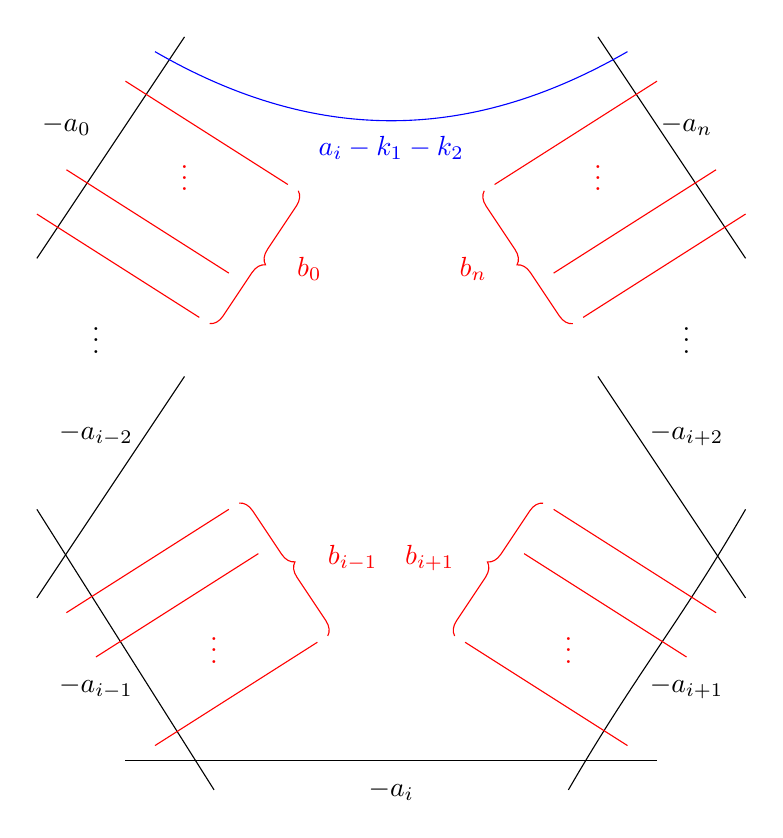
\begin{tikzpicture}[scale= 0.75]\label{figure1}
  % nodes
	\node (0) at (-4.5, -3.5) {};
	\node (1) at (4.5, -3.5) {};
	\node (2) at (-3, -4) {};
	\node (3) at (-6, 0.75) {};
	\node (4) at (3, -4) {};
	\node (5) at (6, 0.75) {};
	\node (6) at (-3.5, 3) {};
	\node (7) at (3.5, 3) {};
	\node (8) at (-6, -0.75) {};
	\node (9) at (6, -0.75) {};
	\node (10) at (-6, 5) {};
	\node (11) at (-3.5, 8.75) {};
	\node (12) at (3.5, 8.75) {};
	\node (13) at (6, 5) {};
	\node (14) at (-4, 8.5) {};
	\node (15) at (4, 8.5) {};
	\node [label={[blue]below:$a_{i} -k_1-k_2$}] (16) at (0, 7.4) {};
	\node [label={above:$-a_0$}] (17) at (-5.5, 6.75) {};
	\node [label={above:$-a_n$}] (18) at (5, 6.75) {};
	\node (20) at (-5, 3.75) {$\vdots$};
	\node (20a) at (5, 3.75) {$\vdots$};
	\node [label={below:$-a_i$}] (21) at (0, -3.5) {};
	\node [label={above:$-a_{i-2}$}] (22) at (-5, 1.5) {};
	\node [label={above:$-a_{i+2}$}] (23) at (5, 1.5) {};
	\node [label={below:$-a_{i-1}$}] (22a) at (-5, -1.75) {};
	\node [label={below:$-a_{i+1}$}] (23a) at (5, -1.75) {};
	%% a_{i-1}
	\node (24) at (-5.5, -1) {};
	\node (25) at (-2.75, 0.75) {};
	\node (26) at (-5, -1.75) {};
	\node (27) at (-2.25, 0) {};
	\node (28) at (-4, -3.25) {};
	\node (29) at (-1.25, -1.5) {};
	\node [red] (30) at (-3, -1.5) {$\vdots$};
	%% a_{i+1}
	\node (31) at (5.5, -1) {};
	\node (32) at (2.75, 0.75) {};
	\node (33) at (5, -1.75) {};
	\node (34) at (2.25, 0) {};
	\node (35) at (4, -3.25) {};
	\node (36) at (1.25, -1.5) {};
	\node [red] (37) at (3, -1.5) {$\vdots$};
	%% a_0
	\node (41) at (-6, 5.75) {};
	\node (42) at (-3.25, 4) {};
	\node (43) at (-5.5, 6.5) {};
	\node (44) at (-2.75, 4.75) {};
	\node (45) at (-4.5, 8) {};
	\node (46) at (-1.75, 6.25) {};
	\node [red] (47) at (-3.5, 6.5) {$\vdots$};
	%% a_n
	\node (49) at (6, 5.75) {};
	\node (50) at (3.25, 4) {};
	\node (51) at (5.5, 6.5) {};
	\node (52) at (2.75, 4.75) {};
	\node (53) at (4.5, 8) {};
	\node (54) at (1.75, 6.25) {};
	\node [red] (55) at (3.5, 6.5) {$\vdots$};
	% edges
	\draw (0.center) to (1.center);
	\draw (6.center) to (8.center);
	\draw (3.center) to (2.center);
	\draw (7.center) to (9.center);
	\draw [in=60, out=-120] (5.center) to (4.center);
	\draw (11.center) to (10.center);
	\draw (12.center) to (13.center);
	\draw [bend right,blue] (14.center) to (15.center);
	%% a_{i-1}
	\draw [red] (24.center) to (25.center);
	\draw [red] (26.center) to (27.center);
	\draw [red] (28.center) to (29.center);
	%% a_{i+1}
	\draw [red] (31.center) to (32.center);
	\draw [red] (33.center) to (34.center);
	\draw [red] (35.center) to (36.center);
	%% a_0
	\draw [red] (41.center) to (42.center);
	\draw [red] (43.center) to (44.center);
	\draw [red] (45.center) to (46.center);
	%% a_n
	\draw [red] (49.center) to (50.center);
	\draw [red] (51.center) to (52.center);
	\draw [red] (53.center) to (54.center);
	% braces
	\draw [decorate,decoration={brace,amplitude=5pt},xshift=5pt,yshift=3pt,red] (-2.75, 0.75) -- (-1.25, -1.5) 
	node [red,midway,xshift=2.5em,yshift=1ex] {$b_{i-1}$};
	\draw [decorate,decoration={brace,amplitude=5pt},xshift=-5pt,yshift=3pt,red] (1.25, -1.5) -- (2.75, 0.75) 
	node [red,midway,xshift=-2.5em,yshift=1ex] {$b_{i+1}$};
	\draw [decorate,decoration={brace,amplitude=5pt},xshift=5pt,yshift=-3pt,red] (-1.75, 6.25) -- (-3.25, 4) 
	node [red,midway,xshift=2em,yshift=-1ex] {$b_0$};
	\draw [decorate,decoration={brace,amplitude=5pt},xshift=-5pt,yshift=-3pt,red] (3.25, 4) -- (1.75, 6.25) 
	node [red,midway,xshift=-2em,yshift=-1ex] {$b_n$};
\end{tikzpicture}
\end{center}
\caption{Example of a minimal surface with invariants $S = [a_1, \, \dots\, a_n]$ and the number of blowups being $k_1$ and $k_2$.\label{fig!logdp}}
\end{figure}


In Figure~\ref{figure1} the picture is where the map to the Hirzebruch surface is an isomorphism on an exceptional curve $E_i$, where $1<i<n$. Here the red curves indicate $-1$-curves and the blue curves indicate curves with positive self-intersection. The blue curve has self-intersection $a_i - k_1- k_2$. This value is dependent on the map to the Hirzebruch surface $\mb{F}_{a_i}$.  If $i=1$ or $i=n$ then we would have a similar looking configuration except with positive curve now having self-intersection $a_i + 2 - k_1$ as we consider the curve in the linear system $|(l+1)F + B|$ which would be the nodal curve \hbox{inside $|{-}K_X|$.} 

The toric degeneration property now follows. By construction all these surfaces $X$ are \LJ s,
and so admit a toric degeneration as mentioned in the technical background \ref{GrossSec}.
%When these singularities are $\mb{Q}$-Gorenstein rigid we get a unique corresponding singularity content, as there is only one surface. 
\end{proof}

\begin{rem}\rm
If for every possible value of $k_1$ and $k_2$ we have $k_1 + k_2 > a_i$ for all $i$. Then there are no log del Pezzo surfaces with singularity $S$. For instance the singularity $S = [3,2,2,2,2,2,2,2,2,2,3]$ cannot be the only singularity on a log del Pezzo surface. This enables us, in certain case, to state existence of a surface in terms of length of the singularity.
\end{rem}
\begin{comment}
\begin{cor}
Let $S$ be a singularity with small discrepancy, $-a_1, \dots , -a_n$ be the self-intersection of the resolutions. Then if $n \geq \max (a_i) + 5 $. Then there exists no \ldp\ with only singularities of type $S$.
\end{cor}
\end{comment}

We use these results to classify \ldp\ surfaces with certain singularities. This leads to the following corollaries in which we classify all log del Pezzo surfaces with singularities of small discrepancy, each of which is resolved by a one or two exceptional curves.
 
\section{Examples}
 
We start by specifying how we deviate from the previous literature. In \cite{ReidSuzuki} they construct cascades as explicit maps between \ldp\ surfaces, mirroring the classical constructions. We do not do this, however we explicitly state when the map exists and give good embeddings. If a variety admits no floating $-1$-curves, so a basic surface, we call it the root of a cascade. If a surface $X$ cannot be blown up at any point while preserving ${-}K_X$ ample we call it the head of a cascade. 


\begin{cor}\label{LengthOne}
Let $X$ be a log del Pezzo surface with small discrepancy and
basket  $\{ \{ \frac{1}{p_1}(1,1), \, \dots \, \frac{1}{p_n}(1,1) \}, \, m \}$
for $n\ge0$ and $m\ge0$. Then $n\le2$ and moreover
\begin{enumerate}
\item\label{dp11i}
if $n\le1$ then either $X$ is a smooth del Pezzo surface or 
lies in a cascade over $\P(1,1,k)$ (see \cite{CP});
\item\label{dp11ii}
if $n=2$ then let $c$ be the highest common factor of $p$ and $q$ and $a = \frac{p}{c}$, $b = \frac{q}{c}$. Then $X$
is isomorphic to a quasismooth weighted hypersurface
$X_{a+b}\subset \mb{P}(1,\,1,\,a,\,b)$ quotiented out by $\mu_c$ acting with weights $(1,1,0,1)$. Conversely any such hypersurface with $p,q\ge4$ is
a log del Pezzo surface with small discrepancy.
\end{enumerate}
In particular, in the case of two singularities there is no cascade.
\end{cor}

The small discrepancy condition is equivalent to the condition that
$p_i \geq 4$ for each $i=1,\dots,n$. 
For the sake of completeness, we outline the classification result of \cite{CP} that
describes part~\ref{dp11i}, which also follows independently from Propostion~\ref{Surfaces to F_1} and Theorem~\ref{ThmOnSing}.

\begin{proof}
With these restrictions on singularities, it fits the criterion for the above theorem. The explicit classification was done in the proof of Theorem~\ref{ThmOnSing}. The case of one singularity was done in \cite{CaveyPrince}. The only examples of these surfaces with more than one singularity are constructed by blowing up a Hirzebruch surface in several points along a line and then contracting the two curves. Denote this surface by $X$. Then $X$ admits a toric degeneration to $(-p_1, -1), \, (0, 1), \, (p_2, 1)$. This is $\mb{P}(a+b, a, b)$ quotiented out by $\mu_c$ acting with weights $(1,1,0,1)$. Taking the $v_{a+b}$ gives us the desired embedding. Note $X$ admits a $\mb{C}^*$ action and the degeneration is equivariant with respect to the torus action. We have $-K_X^2 = \frac{4}{p_1} + \frac{4}{p_2}$. Even in cases where $-K_X^2 > 1$ we see that $X$ cannot be blown up while preserving $-K_X$ ample. If $X$ admitted a blow up at a general point $P$ then there is a fiber $F$ such that $P \in F$. Then $\widetilde F$ is a $-1$-curve on the minimal resolution connecting the $-p_1$ curve with the $-p_2$ curve. This is a contradiction. Hence there is only one element in the cascade.



We note that this surface can be see as a hypersurface of degree $p+q$ inside $\mb{P}(1,\,1,\,p,\,q)$.

\end{proof}
We now do a more difficult example by classifying the \ldp's with singularities $S_{a,b}$ with resolution $E_1, \, E_2$ with $E_1^2 = -a,\, E_2^2 = -b$. To make sure that this obeys they conditions on the theorem we insist $a, \, b \neq 2$. We note that the case of $S_{3,3}$ does satisfy the conditions for the theorem. However we are interested in $\mb{Q}$-Gorenstein smoothings and $S_{3,3}$ is not $\mb{Q}$-Gorenstein rigid and admits a partial smoothing to $\frac{1}{6}(1,1)$ singularity. These were classified above. This is the only one of these singularities which is not $\mb{Q}$-Gorenstein rigid. This is a more complicated example of how the above theorem can be used.


\begin{cor}\label{doublecurve}
Let $X$ be a surface such that the basket is  $(\{ S_{a_1, \, b_1}, \dots , S_{a_m, \, b_m} \}, \, n )$, with the condition that $a_i, \, b_i \geq 3$ and we exclude the case $a_i = b_i = 3$. Then there is at most one singularity $S_{a, \, b}$.


Moreover all such surfaces fall into a cascade of the following form
\[
% https://tikzcd.yichuanshen.de/#N4Igdg9gJgpgziAXAbVABwnAlgFyxMJZABgBpiBdUkANwEMAbAVxiRAA0B9OgPWJAC+pdJlz5CKAIzkqtRizZdekwcJAZseAkQBMM6vWatEIADqmAxlAg4EQkZvFEAzPrlHF3HsDoBaSQIABKoOYtooACykkrKGCiZcKvbqoloSyACs0bHyxhycOiEpjuEkpDo5HgmcAEZ8RRph6dIVBrmedUlqjWm65ZXxZpbWtg2pTiiure6DXHXANf4CgrIwUADm8ESgAGYAThAAtkjSIDgQSGQzeeZoABZYXvzUDHQ1MAwACuPhIAwwOxwRX2RyQejOF0QpziN1M90eyhALzeH2+JQkfwBQOSIOOiFcELBbSqQ3hXh8vh0y2R7y+Pwx-0BwIOeIA7NRzkgAGzEwa3B61eo01H0th7LDrO7YtS4pAADg5kPZ1zY-MenSRfxRdPRYolUuZoMQAE5FfLebCyfNFlTNa9aWimnrJdLdiykFFCSaLaq4QLrUtDXjPZz8T6TGryX4AkGkFkvZ6Yb7Pg87drHb0TOKXSsBEA
\begin{tikzcd}
X_a^0 & X_a^1 \arrow[l, "\phi_a^0"]  & \cdots \arrow[l, "\phi_a^1"]  & X_a^{a-1}  \arrow[l, "\phi_a^{a-2}"] &                                                           &                        \\
      &                              &                               &                                      & X_1 \arrow[ld, "\phi_b^{b-1}"] \arrow[lu, "\phi_a^{a-1}"] & X_2 \arrow[l, "\Phi_1"'] & X_3 \arrow[l, "\Phi_2"']\\
X_b^0 & X_b^1 \arrow[l, "\phi_b^0"'] & \cdots \arrow[l, "\phi_b^1"'] & X_b^{b-1} \arrow[l, "\phi_b^{b-2}"'] &                                                           &                       
\end{tikzcd}
\]
\end{cor}

\begin{proof}

Once again by Theorem~\ref{ThmOnSing} there are two roots of the cascade given by the following two surfaces. These correspond to surfaces constructed by blowing up $\mb{F}_a$ in $b$ points on a fiber and $\mb{F}_b$ in $a$ points on a fiber, then contracting the negative curves. We call these surfaces $X_a$ and $X_b$ respectively.

\[
\resizebox{8.75cm}{5.3125cm}{
\begin{tikzpicture}{s}
    \node (0) at (-2.5, 4) {};
	\node (1) at (-2.5, -4) {};
	\node (2) at (2.5, 4) {};
	\node [label={below:$-b$}] (3) at (2.5, -4) {};
	\node (4) at (4, -2.5) {};
    \node (5) at (-3.75, -2.5) {};
	\node (6) at (-4, 2.5) {};
	\node (7) at (4, 2.5) {};
	\node (8) at (0, 3) {};
	\node [label={$a$}] (9) at (0, 2.5) {};
	\node [label={left:$0$}] (21) at (-2.5, 0) {};
	\node [label={below:$-a$}] (22) at (0, -2.5) {};
	\node (23) at (1.5, 1.5) {};
	\node [label={right:$-1$}] (24) at (4, 1.5) {};
	\node (25) at (1.5, 0.5) {};
	\node [label={right:$-1$}] (26) at (4, 0.5) {};
	\node (27) at (1.5, -1.5) {};
	\node [label={right:$-1$}] (28) at (4, -1.5) {};
	\node (29) at (3, -0.35) {$\vdots$};
	\node [label={$X_a$}] (30) at (0, -5) {};
	% edges
	\draw (0.center) to (1.center);
	\draw (2.center) to (3.center);
	\draw (4.center) to (5.center);
	\draw (6.center) to (7.center);
	\draw (23.center) to (24.center);
	\draw (25.center) to (26.center);
	\draw (27.center) to (28.center);
	% brace
	\draw [decorate,decoration={brace,amplitude=5pt},xshift=-5pt,yshift=0pt]
(1.5,-1.5) -- (1.5,1.5) node [black,midway,xshift=-1em] {$b$};\
\end{tikzpicture}
\hspace{1cm}
\begin{tikzpicture}

    \node (0) at (-2.5, 4) {};
	\node (1) at (-2.5, -4) {};
	\node (2) at (2.5, 4) {};
	\node [label={below:$-a$}] (3) at (2.5, -4) {};
	\node (4) at (4, -2.5) {};
    \node (5) at (-3.75, -2.5) {};
	\node (6) at (-4, 2.5) {};
	\node (7) at (4, 2.5) {};
	\node (8) at (0, 3) {};
	\node [label={$b$}] (9) at (0, 2.5) {};
	\node [label={left:$0$}] (21) at (-2.5, 0) {};
	\node [label={below:$-b$}] (22) at (0, -2.5) {};
	\node (23) at (1.5, 1.5) {};
	\node [label={right:$-1$}] (24) at (4, 1.5) {};
	\node (25) at (1.5, 0.5) {};
	\node [label={right:$-1$}] (26) at (4, 0.5) {};
	\node (27) at (1.5, -1.5) {};
	\node [label={right:$-1$}] (28) at (4, -1.5) {};
	\node (29) at (3, -0.35) {$\vdots$};
	\node [label={$X_b$}] (30) at (0, -5) {};
	% edges
	\draw (0.center) to (1.center);
	\draw (2.center) to (3.center);
	\draw (4.center) to (5.center);
	\draw (6.center) to (7.center);
	\draw (23.center) to (24.center);
	\draw (25.center) to (26.center);
	\draw (27.center) to (28.center);
	% brace
	\draw [decorate,decoration={brace,amplitude=5pt},xshift=-5pt,yshift=0pt]
(1.5,-1.5) -- (1.5,1.5) node [black,midway,xshift=-1em] {$a$};\
\end{tikzpicture}
}
\]
From construction, we see the following formula for the anticanonical degree of $X_a$:
 \[
 -K_{X_a}^2 =8 - b + a \left( 1- \tfrac{b+1}{ab-1} \right) ^2 + b \left(1- \tfrac{a+1}{ab-1} \right)^2 -2\left(1- \tfrac{a+1}{ab-1}\right)\left(1- \tfrac{b+1}{ab-1}\right)
\] 
We note that once we blow up $a$ time our formula will be completely symmetric in $a$ and $b$.

Each of these admit a toric degeneration, to $\mb{P}(1, b, ab-1)$ and $\mb{P}(1, a, ab-1)$ respectively. We can see this as an equivariant toric degeneration of a complexity one variety or via the discrete Legendre transform of section~\ref{Section 2.3}. We only consider the case of $X_a$ since $X_b$ is completely symmetric. We see that we can smooth it by taking the $b$th Veronese embedding and  getting $\mb{P}_{u,\,v,\,w,\,t}(1, 1, ab-1, a)$ with the relation $uw = t^b$. This admits a smoothing giving us the surface lying as $X_{ab} \subset \mb{P}(1,\, 1, \, ab-1, \, a)$. 

We will show that this admits a cascade of length $a+2$. 

The first $a$ terms are easy to describe as we see that these admit a toric degeneration to $X_\Sigma$ with $\Sigma$ being the fan with rays $(-1, b), \, (-1, 0), \, (a, -1), \, (a-u, -1)$, where $u$ is the number of blowups. This has an $A_{b-1}$ singularity and an $A_{u-1}$ singularity. We see that this is the toric degeneration by considering the fan $(-1, a)$, $(0, -1)$, $(1,-1)$ with $a-1$ focus focus singularities along the vector $(1,0)$ and $u$ singularities along the vector $(0,1)$. We can can then compute the dual, via the discrete legendre transform to get the following polygon:
\[
\]
Via Cox rings this can be viewed as $\mb{C}^4_{\{x, y,z,t\}}$ with a quotient 
\[
\begin{blockarray}{cccc}
	x & y & z & t \\[4pt]
      \begin{block}{(cccc)}
		u & 0 & bu - (ab-1) & ab-1 \\
		1 & ab-1 & b & 0 \\
      \end{block}
\end{blockarray}
\]
Taking the Veronese embedding of degree $\begin{binom}{u}{b} \end{binom}$ we get a codimension 2 complete intersection with weights
$\begin{matrix} b & b^2u \\ ab & u \end{matrix}$ 
inside the toric variety with weights

\[
\begin{blockarray}{ccc ccc}
	x^b & y^b & xy & z^u  & t^u & tz \\[4pt]
      \begin{block}{(ccc ccc)}
		b & 0 & 1 & bu - (ab-1) & ab-1 & b\\
		1 & ab-1  & a & u & 0 & 1\\
      \end{block}
\end{blockarray}
\]
We can see the smoothing of both the $A_n$ singularities inside this embedding, so this gives this a good coordinate construction for our variety.

 After $a+1$ blowups the surface admits a toric degeneration to the toric variety defined by the spanning fan of $(-1, b)$, $(-1, -1)$, $(a, -1)$. The toric degeneration after $a+2$ blowups is given by spanning fan $(-1,0)$, $(-a, -1-a)$, $(-1, -1-a)$, $(b, ab-1)$. 

To see the cascade result we note that if you blow up the surface $X_a$ times at points $P_1 \dots P_a$. To each of these points there is a unique fiber $F_i$ passing through it. The strict transform of these fibers after blowing up is a $-1$-curve going through the $-a$-curve. Hence after blowing $X_a$ and $X_b$ respectively $a$ and $b$ times we get a surface which has as a boundary three curves with self-intersection $0, -a, -b$ and in both cases you have your $a$ and your $b$ curves have $a$ and $b$ minus one curves intersecting them respectively. Hence they are isomorphic. We can also see this as an isomorphism of affine manifolds.
 
 
We note that we have made in the above calculations no effort to show that the elements in the cascade are \ldp\ surfaces. However it is not hard to show, assume we are blowing up $a+2$ points giving a surface $X_3$. If this is a \ldp\ surface then every element in the cascade is. This has minimal resolution $Y_3$. The class group of $Y_3$ is generated by the curves $D_1$, $D_2$, $D_3$, $D_4$, $E_1^0, \dots, E_b^0$,  $E_1^1, \dots, E_{a+2}^1$. Here the $D_i$ form a cycle such that $\sum D_i \in |{-}K_{Y_3}|$. These have self-intersections $-a, \, -b, \, -1, \, -1$ respectively. Here $D_3$ was a curve of degree $a$  on $\mb{F}_a$ blown up $a+1$ times and $D_4$ was a fiber on which a single point has been blown up. The $E_i^0$ are $-1$-curves intersecting the $-b$ curve and are not floating. The $E_i^1$ are floating $-1$-curves. We wish to show ${-}K_{X_3}$ is ample. We show $-K_{X_3} \cdot C > 0$ for all $C$ generating the class group which is equivalent. We note that the curves $D_1, \, D_2$ are contracted when sent to $X_3$. We note that ${-}K_{X_3} \cdot E_i^0 = {-}K_{X_a} \cdot E_i^0 > 0$ as we are blowing up points not on these curves and ${-}K_{X_a}$ is ample. Then $-K_{X_3} \cdot E_i^0 = 1$ as these are floating $-1$-curves. Finally to see that $-K_{X_3} \cdot D_3 > 0$ we note that, when pushed forwards to $X_3$, it only goes through the one singularity on $X_3$ with multiplicity $-1$. This is because on $Y_3$ it is only intersecting the $-a$-curve transversely. Hence $-K_{X_3} \cdot D_3 = 1 + d_a$ where $d_a$ is the discrepancy of the $-a$-curve. Via log terminality we have $d_a > -1$. Hence the product is greater than 0. The argument for the curve $D_4$ is symmetric with $d_a$ replaced with $d_b$. From this we see $X_3$ is a \ldp, hence every surface in the cascade is a \ldp\ surface.
\end{proof}

This structure of the cascade can be put in more general terms. 

\section{Cascades}
Given a singularity with small discrepancy such that the minimal resolution is $a_1, \dots a_n$, there are a finite number of basic surfaces classified in Theorem~\ref{ThmOnSing}. Attached to any one of these basic surfaces $X$ with minimal resolution $Y$ we have the following invariants $a_i$ and $k_1$, $k_2$. The $a_i$ indicates that $Y$ admits a map to $\mb{F}_{a_i}$ which is an isomorphism on the negative section. The invariants $k_1$ and $k_2$ are the number of times we blew up general points on $\mb{F}_{a_i}$ to obtain $Y$.

\begin{thm}
Let $X_i$ be one of the basic surfaces constructed in Theorem~\ref{ThmOnSing}. We can describe how their cascades. In the case when the singularities are of the form $\frac{1}{p}(1,1)$ the cascades have been classified by \cite{CP} and the above example. 

For the general case we split in to cases. We label the exceptional curves on $X_i$ arising via the first $k_1+k_2$ blowups by $E_i^S$ and $E_i^T$ respectively. Let $s_i$, $t_i$ be the number of $-1$-curves intersecting $E_i^S$ and $E_i^T$ respectively. We then classify the cascade via these invariants


There is the sporadic case where the singularity is length one where we have the cascade arising in \cite{CP} and the single surface with two singularities.

Outside of the above case, consider $X$ a surface with $k_1$ and $k_2$ not equal to zero. In addition $s_1$, $t_1$, $s_2$ and $t_2$ are all non zero. Then we have the following cascade
\[
\begin{tikzpicture}[baseline= (a).base]
\node[scale=.6] (a) at (0,0){
% https://tikzcd.yichuanshen.de/#N4Igdg9gJgpgziAXAbVABwnAlgFyxMJZABgBoBmAXVJADcBDAGwFcYkQANAAgF4uOA+sRABfUuky58hFAEYK1Ok1btBs0eJAZseAkQBMCmgxZtEIADoWAxlAg4EYiTulFyRpadUDg9ALQA1gKygQL6frIiGs5SeigALB4mKuaCvqEhQfpRTlqSujLI7vGKyWYgAJrReS5xyIYArKXK5RXBAHrqudqxhYlNxi3sbbLt+tU9BQakAGzNXuZWtHYOE-muCbPzKZYWy-aOmpMb9aQA7NutPmDBIp1rtX3nl8PXYXfj3et1DaSyL6kAOSAnz0YEZcFZcGRB69IgzUj6AGVYGwqYoBHEZEcYGgyHBfH6cHZNEnM6kLGDBa7WwHUl1AAcFOxuOEX0eRHJ-ypO2AI06IlR7LhKHJSJ55T5HWyQqO30KTO5nh2Vlpq2F6OQTPFyvKqpWhximoAnH9kVLgDdZFxgXdIsCuPTCqadWV2BabkTAR9BYCnURfgNdaoQb5ARDQkSIjk5RyMaQShLhn6NScEXMk6k8RGoX4Zf7RVtMzSDQWtUXg0ChGXyUG3eYpaN7TWE+b+fnU4zSHWhosbKXOwrW8X9XTB0RTYnKyAPWFvWNBWXTT3qbPZPPmyJFDAoABzeBEUAAMwAThAALZIeQgHAQJBkStgZiMRg0Rj0ABGMEYAAV5exGBgI8cGqU8LyQQwbzvRBr3rJ8XzfT9vz-OMQEA4DQLPS9EHcKCIMzeDXzQpDf3-cx0JA3IwOw3DbyQX5H2fIj3y-UjUIozDwMQRI8JwgimMQ1iUJFNCgMozRqPomg6MQBFGIQ4ihLI0SMKorCpN48l5OYkjhPRFTxOPdTZOk6CmW0wTkOUji1K4rSZNNCzFKs9ixM47DzJk2QHzggTnLYkSbIk4zHK82De0IyyAv0oKjK4nivOyYKuNkSCvPIWzsNS0yr3iTLcpymCGnyorCtkGYStkWjoNkM5Kuqq8GUqzzoP0YgSrawr9CSuKstC1rImSrL7Jq40SoS1qMqGiCGsQfQ8umubZv0YrFpWrqKrWuSZP0Oq1omiCmv2rqxrWlqkHIdq1v6i7Bt627CvIHqQEknCHxk8gMsoEQgA
\begin{tikzcd}
        &               &                  &                                     &                                                 &                                               & X''_{a''-k_1''-k_2''-2} \arrow[r] & \cdots \arrow[r]    & X''_0            &                   \\
        &               &                  &                                     &                                                 & X''_{a''-k_1''-k_2''-1} \arrow[rd] \arrow[ru] &                                   & {Y_1^1}'' \arrow[r] & \cdots \arrow[r] & {Y_{n_1 ''}^1}''  \\
        &               &                  &                                     &                                                 &                                               & Y'' \arrow[ru] \arrow[r]          & {Y_1^2}'' \arrow[r] & \cdots \arrow[r] & {Y_{n_2''}^2}''   \\
X = X_0 & X_1 \arrow[l] & \cdots \arrow[l] & X_{a-k_1-k_2-1} \arrow[l] \arrow[d] & X_{a-k_1-k_2} \arrow[l] \arrow[ruu] \arrow[rdd] &                                               &                                   &                     &                  &                   \\
        &               &                  & Y \arrow[ld] \arrow[rd]             &                                                 &                                               & Y' \arrow[rd] \arrow[r]           & {Y_1^2}' \arrow[r]  & \cdots \arrow[r] & {Y_{n_2'}^2}'     \\
        &               & Y_1^1 \arrow[d]  &                                     & Y_1^2 \arrow[d]                                 & X'_{a'-k_1'-k_2'-1} \arrow[ru] \arrow[rd]     &                                   & {Y_1^1}' \arrow[r]  & \cdots \arrow[r] & {Y_{n_1'}^1}'     \\
        &               & \vdots \arrow[d] &                                     & \vdots \arrow[d]                                &                                               & X_{a'-k_1'-k_2'-2}' \arrow[r]     & \cdots \arrow[r]    & X'_0             &                   \\
        &               & Y_{n_1}^1        &                                     & Y_{n_2}^2                                       &                                               &                                   &                     &                  &                  
\end{tikzcd}
};
\end{tikzpicture}
\]
where we have 
\begin{enumerate}
\item $X$ is a surface with $k_1$ and $k_2$ not equal to zero. In addition $s_1$, $t_1$, $s_2$ and $t_2$ are all non zero.


\item The $Y_{n_1}^1$ or $Y_{n_2}^2$ are surfaces such that $k_1 = 0$ and $k_2 = a_1 + 1 - s_1$ or $k_2 = a_1 + 1 - t_1$ respectively. In each of the $Y_i$ there is only one degenerate fiber in the $\mb{P}^1$ fibration induced by the map to the Hirzebruch surface. 

\item The surfaces $X_0'$ and $X_0''$ are of the same form as $X$ and the picture has 3-fold symmetry.
\end{enumerate}
There are a variety of subcases of this which occur 
\begin{enumerate}
\item The next case is $X$ is a surface with $k_1 = k_2 = 0$ and there two non general fibers or $s_2 = t_2 = 0$. Then the cascade is 
\[
% https://tikzcd.yichuanshen.de/#N4Igdg9gJgpgziAXAbVABwnAlgFyxMJZABgBpiBdUkANwEMAbAVxiRAA0ACAXk-YH1iIAL6l0mXPkIoAjOSq1GLNgJkixIDNjwEiAJnnV6zVohAAdcwGMoEHAlHjtUogGZDikyv7A6AWgBrfhlA-j0-GWF1J0ldFAAWD2NlMwFfUJCgvSjHTQkdaWR3GQVk0xAATWi85zjkAz1SpXKK4IA9NVytWMLExqNmtlaZNr1q7oL9UlcmrzNLGlt7cfyXBOnZlItzRbsHDQm1+tJ4zZafMGDhDpXa3pOzoYuw67Gu1bqAViTB1IByHx0P4ZYFZYGREQKGBQADm8CIoAAZgAnCAAWyQchAOAgSDInhSYCYDAY1AYdAARjAGAAFD7SEAMGCInDVFHopAGbG4xBYspIIkksmU6l0u5sJkstmojGIdzczkDOaC0mMkW0+kS5ms3Ls2XynFIb4E0wq4VUjXisySnUaPVIRIKuVKwnE1Xki1inpaqW6mVG6iGxAANhdprd5tFmut2ulHMQxqDAHYwwKI2rPdHGbG-fHQ06ABypxBmjNRq3Z312-2IFNOgCcxdLHvL3pjVaRNaLTpk+P5JfTLctbcrts78cbPb5v2b6q9k3bY5A9sQjqDMmyFGEQA
\begin{tikzcd}
X = X_0 & X_1 \arrow[l] & \cdots \arrow[l] & X_{a-k_1-k_2-1} \arrow[l] \arrow[d] & X_{a-k_1-k_2} \arrow[l]  &  \\
        &               &                  & Y \arrow[ld] \arrow[rd]             &                                   &                     \\
        &               & Y_1^1 \arrow[d]  &                                     & Y_1^2 \arrow[d]                   &                     \\
        &               & \vdots \arrow[d] &                                     & \vdots \arrow[d]                  &                     \\
        &               & Y_{n_1}^1        &                                     & Y_{n_2}^2                         &                    
\end{tikzcd}
\]
\item The next case is $X$ is a surface with $k_1 = 0$, $k_2 \neq 0$ and there are two non general fibers or $t_2 = 0$. 
\[
% https://tikzcd.yichuanshen.de/#N4Igdg9gJgpgziAXAbVABwnAlgFyxMJZABgBoBGAXVJADcBDAGwFcYkQANAAgF4uOA+sRABfUuky58hFOQrU6TVu0HlR4kBmx4CRAEzyaDFm0QgAOuYDGUCDgRiJ26UQDMhxSZUDg9ALQA1gLkgQJ6fuQi6k5SuigALB7GymaCvqEhQXpRjpqSOjLI7noKyaYgAJrRec5xyAaupUrlFcEAemq5WrGFiY1Gzeyt5G161d0F+qTxTV5mlrS29uP5LgnTsykW5ot2DhoTa-WkAKybLT5gwSIdK7W9p+dDl2E3Y12rdSdJg6kA5D56H8MsCssDIncekQAGykYhPMwVP6QyYoADscIRIGAw1GImRH3uRAAHJiBnNtjY9iijgBOMmeLY4l56P5vfE0ur0qjkpmtYBXchsjocwlQ9E-CnMkaRAkHT6FUk8xnlSxU5Zi1HIWElXnlNJAkGhVl+bJymJajG6lXsNVLfYWo6k61lFQA4QiBQwKAAc3gRFAADMAE4QAC2SDkIBwECQZBtiDAzEYjBojHoACMYIwAAoK9iMGCBnDVEPhpAGaOxxBR12J5OpkDprO5-NmQvF0uhiOIdxVit6pBJlNpzPZvNE9tFku5Ms9vsxpDfBPDxvN8dtpvTrvlxCJfu9wf1kdNsetydbzuz7tLmiLxCwlcN0ctifiy8zjRz28HjFPk-rue74dp+QY3g+d7VqS-5rmeb6oh+O49n+970jBL4bheIFIUg0H3uQ8Z1quGFAQh2HXruaH4bWvzEaer6buRX7gfu+HZMxu7kJW956MQFE9rxkEVpEHECVGPHsWBnHcdW5CuPxkYLrJ8QKTWrGyScqnkMu+HQlpVGyWiWlKZGxKeiIQA
\begin{tikzpicture}[baseline= (a).base]
\node[scale=.6] (a) at (0,0){
\begin{tikzcd}
        &               &                  &                                     &                                   &                                           & Y' \arrow[r] \arrow[rd]       & {Y_1^2}' \arrow[r] & \cdots \arrow[r] & {Y_{n_2'}^2}' \\
X = X_0 & X_1 \arrow[l] & \cdots \arrow[l] & X_{a-k_1-k_2-1} \arrow[l] \arrow[d] & X_{a-k_1-k_2} \arrow[l] \arrow[r] & X'_{a'-k_1'-k_2'-1} \arrow[rd] \arrow[ru] &                               & {Y_1^1}'           & \cdots \arrow[r] & {Y_{n_1'}^1}' \\
        &               &                  & Y \arrow[ld] \arrow[rd]             &                                   &                                           & X_{a'-k_1'-k_2'-2}' \arrow[r] & \cdots \arrow[r]   & X'_0             &               \\
        &               & Y_1^1 \arrow[d]  &                                     & Y_1^2 \arrow[d]                   &                                           &                               &                    &                  &               \\
        &               & \vdots \arrow[d] &                                     & \vdots \arrow[d]                  &                                           &                               &                    &                  &               \\
        &               & Y_{n_1}^1        &                                     & Y_{n_2}^2                         &                                           &                               &                    &                  &              
\end{tikzcd}
};
\end{tikzpicture}
\]
\item The next case is $s_1 = 0$ and two non general fibers
\[
% https://tikzcd.yichuanshen.de/#N4Igdg9gJgpgziAXAbVABwnAlgFyxMJZABgBoBGAXVJADcBDAGwFcYkQANAAgF4uOA+sRABfUuky58hFOQrU6TVu0HlR4kBmx4CRAEzyaDFm0QgAOuYDGUCDgRiJ26UQDMhxSZUDg9ALQA1gLkgQJ6fuQi6k5SuigALB7GymaCvqEhQXpRjpqSOjLI7noKyaYgAJrRec5xyAaupUrlFcEAemq5WrGFiY1Gzeyt5G161d0F+qTxTV5mlrS29uP5LgnTsykW5ot2DhoTa-WkAKybLT5gwSIdK7W9p+dDl2E3Y12rdSdJg6kA5D56H8MsCssDIncekQAGykYhPMwVP6QyYoADscIRIGAw1GImRH3uRAAHJiBnNtjY9iijgBOMmeLY4l56P5vfE0ur0qjkpmtYBXchsjocwlQ9E-CnMkaRAkHT6FUk8xnlSxU5Zi1HIWElXnlNJAkGhVl+bJymJajG6lXsNVLfYWo6k61lFQA4QiBQwKAAc3gRFAADMAE4QAC2SDkIBwECQZBtiDAzEYjBojHoACMYIwAAoK9iMGCBnDVEPhpAGaOxxBR12J5OpkDprO5-NmQvF0uhiOIdxVit6pBJlNpzPZvNE9tFku5Ms9vsxpDfBPDxvN8dtpvTrvlxCJfu9wf1kdNsetydbzuz7tLmiLxCwlcN0ctifiy8zjRz28HjFPk-rue74dp+QY3g+d7VqS-5rmeb6oh+O49n+970jBL4bheIFIUg0H3uQ8Z1quGFAQh2HXruaH4bWvzEaer6buRX7gfu+HZMxu7kJW956MQFE9rxkEVpEHECVGPHsWBnHcdW5CuPxkYLrJ8QKTWrGyScqnkMu+HQlpVGyWiWlKZGxKeiIQA
\begin{tikzpicture}[baseline= (a).base]
\node[scale=.6] (a) at (0,0){
\begin{tikzcd}
        &               &                  &                                     &                                   &                                           & Y' \arrow[r] \arrow[rd]       & {Y_1^2}' \arrow[r] & \cdots \arrow[r] & {Y_{n_2'}^2}' \\
X = X_0 & X_1 \arrow[l] & \cdots \arrow[l] & X_{a-k_1-k_2-1} \arrow[l] \arrow[d] & X_{a-k_1-k_2} \arrow[l] \arrow[r] & X'_{a'-k_1'-k_2'-1} \arrow[rd] \arrow[ru] &                               & {Y_1^1}'           & \cdots \arrow[r] & {Y_{n_1'}^1}' \\
        &               &                  & Y \arrow[ld] \arrow[rd]             &                                   &                                           & X_{a'-k_1'-k_2'-2}' \arrow[r] & \cdots \arrow[r]   & X'_0             &               \\
        &               & Y_1^1 \arrow[d]  &                                     & Y_1^2 \arrow[d]                   &                                           &                               &                    &                  &               \\
        &               & \vdots \arrow[d] &                                     & \vdots \arrow[d]                  &                                           &                               &                    &                  &               \\
        &               & Y_{n_1}^1        &                                     & Y_{n_2}^2                         &                                           &                               &                    &                  &              
\end{tikzcd}
};
\end{tikzpicture}
\]
\item The next case is $s_1 = t_1 = 0$ and two non general fibers
\[
\begin{tikzcd}
X = X_0 & X_1 \arrow[l] & \cdots \arrow[l] & X_{a-k_1-k_2-1} \arrow[l] & X_{a-k_1-k_2} \arrow[l]  &  \\
\end{tikzcd}
\]
\item We also have the case $s_2 =0$ or $k_1 = k_2 = 0$ with one non general fiber, which has cascade
\[
\begin{tikzcd}
X_a^0 & X_a^1 \arrow[l ]  & \cdots \arrow[l]  & X_a^{a-1}  \arrow[l] &                                                           &                        \\
      &                              &                               &                                      & X_1 \arrow[ld] \arrow[lu] & X_2 \arrow[l] & X_3 \arrow[l]\\
X_b^0 & X_b^1 \arrow[l] & \cdots \arrow[l] & X_b^{b-1} \arrow[l] &                                                           &                       
\end{tikzcd}
\]
\item finally case $s_1 = s_2 =0$ with one non general fiber, which has cascade 
\[
\begin{tikzcd}
X = X_0 & X_1 \arrow[l] & \cdots \arrow[l] & X_{n-1} \arrow[l] & X_{n} \arrow[l]  &  \\
\end{tikzcd}
\]
\end{enumerate}
We note that $s_1=0$ and $s_2 = 0$ with one non general fiber would occur in case 3 above.



\end{thm}
\begin{proof}
Given a singularity $S$ of small discrepancy with length $m>1$. Then a basic surface $X$ with singularity $S$ has minimal resolution $Y$. The surface $Y$ is constructed by taking a Hirzebruch surface $\mb{F}_{a_i}$ picking two points $P_1$, $P_2$ and blowing them up $k_1$ and $k_2$ times, this gives rise to an intermediate surface $Z$ and then $X$ is constructed by doing further blow ups. We can assume $k_1 \leq k_2$ and this gives the relations that either $k_1 = k_2 = 0$ and $m \in \{1, \, 2, \, 3 \}$ or $k_1 = 0$ and $k_1 = m-2$ or $k_1 + k_2 = m-3$. These cases arise by considering the case where the strict transform of both/ one/ none of the fibers are exceptional curves. The case where no fiber becomes an exceptional curve has been classified in Corollary~\ref{LengthOne} and we will note mention it further.


We note that $k_1$ and $k_2$ should not be viewed as invariant of the surface $X$ but an invariant of the given map to $\mb{F}_{a_i}$:
\[
% https://tikzcd.yichuanshen.de/#N4Igdg9gJgpgziAXAbVABwnAlgFyxMJZABgBpiBdUkANwEMAbAVxiRAA0QBfU9TXfIRQBGclVqMWbAJrdeIDNjwEiAJjHV6zVohAAdPQFsARsABiXAPrA6lrF27iYUAObwioAGYAnCIaSiIDgQSMQ8Xr7+iIHBSOoS2mwGaFiOXEA
\begin{tikzcd}
X & Y \arrow[l, "f"] \arrow[r, "\pi"] & \mb{F}_{a_i}
\end{tikzcd}
\]
This is because the map to a Hirzebruch surface is non unique even with the moderate restrictions we have placed on these maps.


We now note that by construction in the case where the strict transform of both fibers are exceptional curves we get a curve $C$ on $Y$ with self-intersection $a_i - k_1 -k_2$. Via construction $C$ was a toric curve and $f_*(C) \in |-K_X|$. We have that the class group of $X$ is generated by $C$ and $D_i$ where $D_i$ are the curves arising from the non toric blowups of $Y$. This implies that the cascade of $X$ is of length $L = a_i - k_1-k_2$  as blowups in general position do not affect the $-K_X \cdot D_i$ and when we blow up $a_i - k_1 -k_2 +1$ times $K_X^2 \leq 0$ via the small discrepancy condition. If $L < 0$ then this surface is not a \ldp\ surface.


In the case where one of the fibers is not exceptional, so $k_2  = 0$,  we have that the class group is generated by the same $D_i$, the fiber class $F$ and a final curve $C$. Here $-K_X = C + F$ and $F^2 = 0$, $C^2 =  a_i - k_1$. This surface admits a cascade of length $L = a_i - k_1 + 2$. This is because, we only need to calculate the intersections on the subgroup generated by $C$ and $F$. If we blowup $L$ times we can assume that we blew up one point on the fiber $F$ and $a_i-k_1+1$ points on the curve $C$. After this process the strict transform of both these curves would have self-intersection $-1$. As these are both on through a singularity with multiplicity one we see that $-K_X$ has positive intersection with these curves. If we blow up one more time we can assume all $L+1$ points lie on a curve in the class $|C+F|$ this has self-intersection $L$ and hence after all these blowups would be a $-1$-curve intersecting the singularity twice. This would not be a \ldp\ surface via small discrepancy.


We now wish to explore the birational relationships between these surfaces. The first stage is to show that the only possible $-1$-curves on any basic surface arise from the class $|B+ a_i F|$ on the Hirzebruch surface $\mb{F}_{a_i}$. To show this we note that it is impossible for any curve that intersects $|B|$ to end up being a floating curve as it will always intersect the curve $B$. So any floating curve $C$ lies in the class $n|B+a_i F|$. To show that $n=1$ we compute the self intersection of these curves. If $n=2$ then the smallest possible self intersection of a curve not going through the singularity  is $4a_i - k_1 - k_2 - 4$ if there are two non general fibers and $4a_i - k_1 -2$ if there is only one. As in the first case $L = a_i- k_1-k_2$ as $a_i \geq 2 $  we have $4a_i -k_1-k_2 - 4 > L$ so we cannot blow up enough to make this a $-1$-curve. In the second case $L = a_i -k_1+2$ so once again as $a_i \geq 2$  we cannot blow up enough to make it a $-1$-curve. As $n$ increases the size of the self intersection increases and hence they can never occur as floating $-1$-curves.


Now we explicitly state how the cascade structure occurs. We note that we can restrict our analysis to the exceptional curves $E_i \subset Y$ that arose as part of the original $k_1$ and $k_2$ blowups. These are the only curves that can be intersected by curves in the class $|B + a_i F|$ as otherwise they would have to intersect the fiber with multiplicity greater than $1$. Label these exceptional curves $S_1, \dots ,S_{k_1}$ and $T_1, \dots , T_{k_2}$ with $S_{1}$ and $T_{1}$ being the strict transforms of the fibers. Hence any potential floating curve intersects a $-1$-curve coming out of a curve $S_i$ and a $-1$-curve coming out of $T_j$. We now denote by $C_{i,\, j}$ the curve intersecting a $-1$-curve coming from $S_i$ and a $-1$-curve coming from $T_j$. Then in the case of both fibers becoming exceptional curves $C_{i, \, j}^2 = L- 4 + i + j$ so in order for it to become a $-1$-curve it needs to be blown up in $L - 3 + i + j$ points. However as the length of the cascade is $L$ this implies $i+j \leq 3$. So $\{ (i, \, j) \} = \{(1,1), (1,2), (2,1) \} $. We now go on a case by case analysis:


\textbf{Case 1}: We start with $(i, \, j)  = (1,\, 1)$. It takes $L - 1$ blowups for these curves to become $-1$-curves. Denoting the number of $-1$-curves intersecting $S_1$ and $T_1$ by $s, \, t$, we label these curves $D_u^S$ and $D_v^T$ respectively. We have $st$ possible curves which would give rise to a $-1$-curve after $L-1$ blowups. We denote by $C_{u, \, v}$ the curve intersecting $D_u^S$ and $D_v^T$. These curves originally lay in $|B+ a_i F|$ so on the Hirzebruch surface they intersected $b$ times. By repeating the same calculation on  this on $Y$ blown up $L-1$ times, we see that $C_{u,\, v}$ intersects $C_{u' , \, v'}$ if and only if $u \neq u'$ and $v \neq v'$. So fixing $C_{u, \, v}$ we get the curve configuration in Figure~\ref{CurveConfigFigure}

\begin{figure}[h]
\resizebox{10cm}{10cm}{
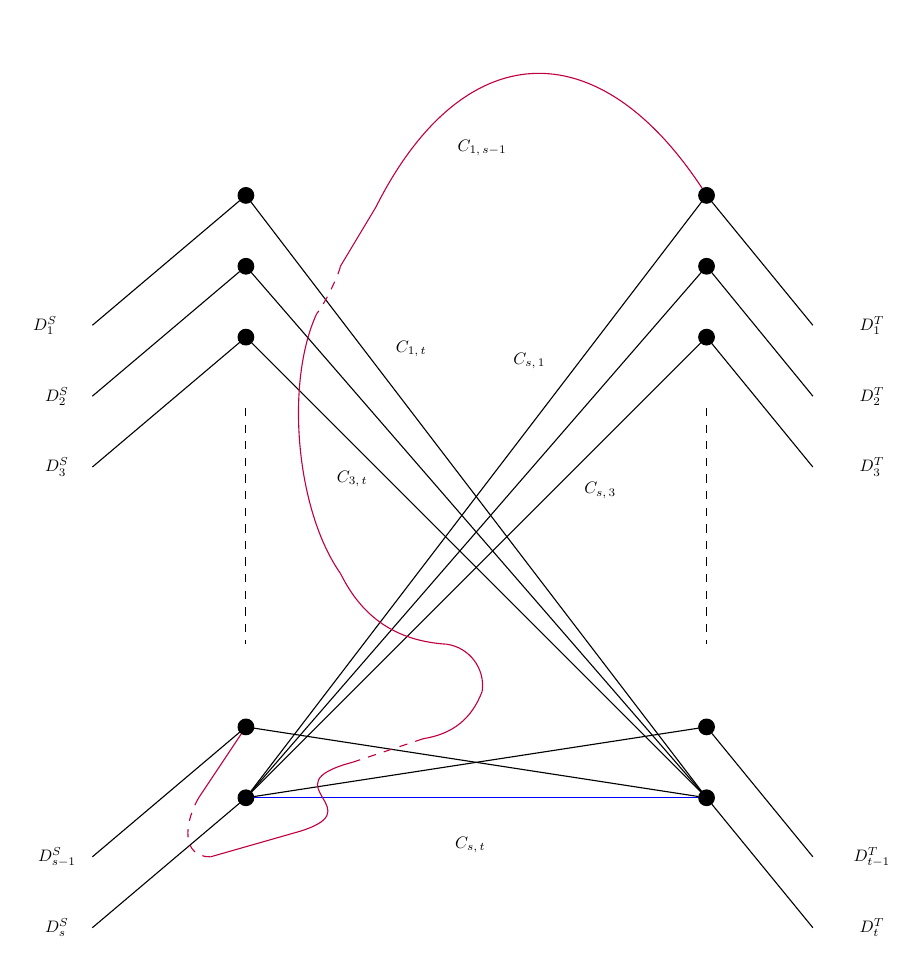
\begin{tikzpicture}[thick,scale=0.6, every node/.style={transform shape}]
	\begin{pgfonlayer}{nodelayer}
		\node [style=Filled Basic] (0) at (0.25, 9.25) {};
		\node [style=Filled Basic] (1) at (0.25, 7.75) {};
		\node [style=Filled Basic] (2) at (0.25, 6.25) {};
		\node [style=none] (3) at (0.25, 4.75) {};
		\node [style=none] (4) at (0.25, -0.25) {};
		\node [style=Filled Basic] (5) at (0.25, -2) {};
		\node [style=Filled Basic] (6) at (0.25, -3.5) {};
		\node [style=Filled Basic] (7) at (10, 9.25) {};
		\node [style=Filled Basic] (8) at (10, 7.75) {};
		\node [style=Filled Basic] (9) at (10, 6.25) {};
		\node [style=none] (10) at (10, 4.75) {};
		\node [style=none] (11) at (10, -0.25) {};
		\node [style=Filled Basic] (12) at (10, -2) {};
		\node [style=Filled Basic] (13) at (10, -3.5) {};
		\node [style=none] (24) at (-3, 6.5) {};
		\node [style=none] (25) at (-3, 5) {};
		\node [style=none] (26) at (-3, 3.5) {};
		\node [style=none] (27) at (-3, -4.75) {};
		\node [style=none] (28) at (-3, -6.25) {};
		\node [style=none] (29) at (12.25, 6.5) {};
		\node [style=none] (30) at (12.25, 5) {};
		\node [style=none] (31) at (12.25, 3.5) {};
		\node [style=none] (32) at (12.25, -4.75) {};
		\node [style=none] (33) at (12.25, -6.25) {};
		\node [style=none] (34) at (3, 9) {};
		\node [style=none] (35) at (2.25, 7.75) {};
		\node [style=none] (36) at (1.75, 6.75) {};
		\node [style=none] (37) at (2.25, 1.25) {};
		\node [style=none] (44) at (-3.75, 6.5) {};
		\node [style=none] (45) at (-3.75, 5) {};
		\node [style=none] (46) at (-3.75, 3.5) {};
		\node [style=none] (47) at (-3.75, -4.75) {$D_{s-1}^S$};
		\node [style=none] (48) at (-3.75, -6.25) {$D_s^S$};
		\node [style=none] (50) at (-3.75, 5) {$D_2^S$};
		\node [style=none] (51) at (-3.75, 3.5) {$D_3^S$};
		\node [style=none] (54) at (-4, 6.5) {$D_1^S$};
		\node [style=none] (55) at (13.5, 6.5) {};
		\node [style=none] (56) at (13.5, 5) {};
		\node [style=none] (57) at (13.5, 3.5) {};
		\node [style=none] (58) at (13.5, -4.75) {$D_{t-1}^T$};
		\node [style=none] (59) at (13.5, -6.25) {$D_t^T$};
		\node [style=none] (60) at (13.5, 5) {$D_2^T$};
		\node [style=none] (61) at (13.5, 3.5) {$D_3^T$};
		\node [style=none] (62) at (13.5, 6.5) {$D_1^T$};
		\node [style=none] (63) at (5.25, 10.25) {};
		\node [style=none] (64) at (5.25, 10.25) {$C_{1, \, s-1}$};
		\node [style=none] (65) at (12.25, -4.75) {};
		\node [style=none] (66) at (4.5, -0.25) {};
		\node [style=none] (67) at (5.25, -1.25) {};
		\node [style=none] (68) at (4, -2.25) {};
		\node [style=none] (69) at (2.5, -2.75) {};
		\node [style=none] (70) at (1.25, -4.25) {};
		\node [style=none] (71) at (-0.5, -4.75) {};
		\node [style=none] (72) at (-0.75, -3.5) {};
		\node [style=none] (73) at (3.75, 6) {$C_{1, \, t}$};
		\node [style=none] (74) at (2.5, 3.25) {};
		\node [style=none] (75) at (6.25, 5.75) {$C_{s, \, 1}$};
		\node [style=none] (76) at (7.75, 3) {$C_{s, \, 3}$};
		\node [style=none] (77) at (5, -4.5) {};
		\node [style=none] (78) at (5, -4.5) {$C_{s,\,t}$};
		\node [style=none] (79) at (2.5, 3.25) {$C_{3, \, t}$};
	\end{pgfonlayer}
	\begin{pgfonlayer}{edgelayer}
		\draw [style=Filled Blue] (6) to (13);
		\draw (6) to (12);
		\draw (5) to (13);
		\draw (2) to (13);
		\draw (1) to (13);
		\draw (0) to (13);
		\draw (6) to (9);
		\draw (8) to (6);
		\draw (7) to (6);
		\draw [style=Dashed Black] (3.center) to (4.center);
		\draw [style=Dashed Black] (10.center) to (11.center);
		\draw (24.center) to (0);
		\draw (25.center) to (1);
		\draw (26.center) to (2);
		\draw (27.center) to (5);
		\draw (28.center) to (6);
		\draw (33.center) to (13);
		\draw (9) to (31.center);
		\draw (8) to (30.center);
		\draw (7) to (29.center);
		\draw [style=Red, bend right=60, looseness=1.50] (7) to (34.center);
		\draw [style=Red] (34.center) to (35.center);
		\draw [style=Red, bend right, looseness=0.75] (36.center) to (37.center);
		\draw [style=new edge style 0, bend left=15, looseness=0.50] (35.center) to (36.center);
		\draw (12) to (65.center);
		\draw [style=Red] (5) to (72.center);
		\draw [style=Red] (71.center) to (70.center);
		\draw [style=Red, in=-165, out=15, looseness=2.50] (70.center) to (69.center);
		\draw [style=Red, bend right] (68.center) to (67.center);
		\draw [style=Red, bend left=45] (66.center) to (67.center);
		\draw [style=Red, bend left] (66.center) to (37.center);
		\draw [style=new edge style 0, in=-180, out=-120, looseness=1.25] (72.center) to (71.center);
		\draw [style=new edge style 0] (69.center) to (68.center);
	\end{pgfonlayer}
\end{tikzpicture}
}
\caption{This is currently not correct, fix the intersection}
\label{CurveConfigFigure}
\end{figure}
Hence if we choose a floating $-1$-curve $C_{u, \, v}$ to contract the only remaining floating curves are $C_{u, \, \beta}$ and $C_{\alpha , \, v}$ where $\alpha \in \{ 1, \dots, s\}$ and $\beta \in \{1 , \dots , t \}$. When the second floating curve is contracted this uniquely defines whether we are iterating over $s$ or over $t$. So after two contractions the cascade is uniquely defined. To see where it ends up we note that a basic surface is uniquely defined by the number of $-1$-curves coming out of each curve on the boundary. Picking one of these chains of  leads to either $s$ blowdowns or $t$ blowdowns. These cases behave symmetrically, so focusing on the case of $s$ blowdowns we get a curve $S_1 = E_1 \subset Y$ with self intersection $-a_1$ and no $-1$-curves coming out of it. So it admits a map to $\mb{F}_{a_1}$. We note that in our notation the basic surface $Y^1_{n_1}$ which it blows down to has to have new value $k^{Y^1_{n_1}}_1 = 0$ as there is only one exceptional curve intersecting it. Hence there is only one non general fiber of the fibration. As we are doing $s$ blow downs the self intersection of the positive section is $1 + s = a_1 - k^{Y^1_{n_1}}_2  + 2$. This gives us $k^{Y^1_{n_1}}_2  = a_1 + 1 - s$. 

\textbf{Case 2}: The second case is $(i, \, j) = (1, \, 2)$. We do not spell this out in the same level of detail. Replicating the above arguments we see that we now get exactly the same curve configuration as in Figure 2 except now connecting the curves $E_1^S$ to $E_2^T$. So once again this leads to a set of two branching contractions. However the choice of contractions now give different basic surfaces at the end. If you contract the curves $C_{u, \,1}$ you get a surface $Z_{m_1}$ with $k^{Z_{m_1}}_1 = 0$ and only one non general fiber. However now via the same calculations as previously $k^{Z_{m_1}}_2 = a_1 + 2 - s$. In the other case we are contracting all curves of the form $D^T_v$ this gives rise to a surface $W_{m_2}$ with $k_1 = 0$ but two exceptional fibers. This has invariant $k_2^{W_{m_2}} = t$. 

\textbf{Case 3}: The final case is $(i, \, j) = (2, \, 1)$. This is symmetrical to case 2.

A crucial point in this proof is that each case behaves independently of the others as two floating curves don't intersect each other only if they lie in the same case. This means that upon any contraction we have limited ourselves to a set of $-1$-curves.

We note that if there are no $-1$-curves coming out of the curves $E_1^S$ and $E_1^T$ then the cascade is a straight line as the above discussion is entirely predicated on their existence.
Via similar logic we get the following cases where not all of these maps occur. Let $s_i$, $t_i$ equal the number of $-1$-curve going through $E_i^S$ and $E_i^T$ respectively. These conditions are symmetrical in $s$ and $t$
\begin{enumerate}
\item $k_1 = k_2 = 0$ and there two non general fibers or $s_2 = t_2 = 0$. Then neither case 2 or 3 can occur.

\item $k_1 = 0$, $k_2 \neq 0$ and there are two non general fibers or $t_2 = 0$. Then case 3 cannot occur.

\item $s_1 = 0$. Then case 1 and 2 cannot occur. 

\item $s_1 = t_1 = 0$ or $s_1 = s_2 = 0$. Then the cascade is a straight line. 
\end{enumerate}
This concludes the cascade for basic surfaces of this type. 

We make a quick mention of what happens in the case where there is only one non generic fiber. These surfaces all start by blowing up a point $k$ times. Label the exceptional curves that arose from blowing up this point $E_{k}, \dots E_1$ and we denote the strict transform of the fiber by $E_{0}$. Once again $L = a_1 - k+ 2$ and we have curves with self intersection $a_1 - i -1$ intersecting the $-1$-curves coming out of $E_i$. To get a $-1$-curve we need $a_1 - i - 1 < L = a_1 - k+2$ giving $k-i < 3$ so $i \in \{ k, \, k-1,\, k-2 \}$. 

Considering the case where $i = k-1$ then the curve intersects a $-1$-curve going through the curve $E_{k-1}$, which has self intersection $-a_{k-1}$. Blowing down all these floating curves gives rise to a basic surface $X$ which has a map to $\mb{F}_{a_{k-1}}$, sending $E_k$ to the negative section. Hence this is a surface in one of the above cases, as there are two exceptional curves adjacent to the negative section. So we it lies in one of the above diagrams.
\end{proof}

The smallest possible length of a singularity where this full cascade can be seen is if the singularity is length 5 or more.

\section{Outside of the small discrepancy}

If you consider singularities of the type $\frac{1}{p}(1,1)$ we note that if $p \geq 7$ then a $\frac{1}{p}(1,1)$ singularity cannot be joined to any other $\frac{1}{p}(1,1)$ singularity by a $-1$-curve. Hence a similar analysis to  Theorem~\ref{ThmOnSing} gives us the bound that there cannot be a \ldp\ surface $X$ with singularities $\frac{1}{p_1}(1,1), \, \dots, \, \frac{1}{p_n}(1,1)$ and $p_1 \geq 7$ and more than 2 different singularities.

However when we enter the case where $p_1 < 7$ you can get surfaces with many more singularities. For instance consider the surface $X$ with the following minimal resolution:
\[
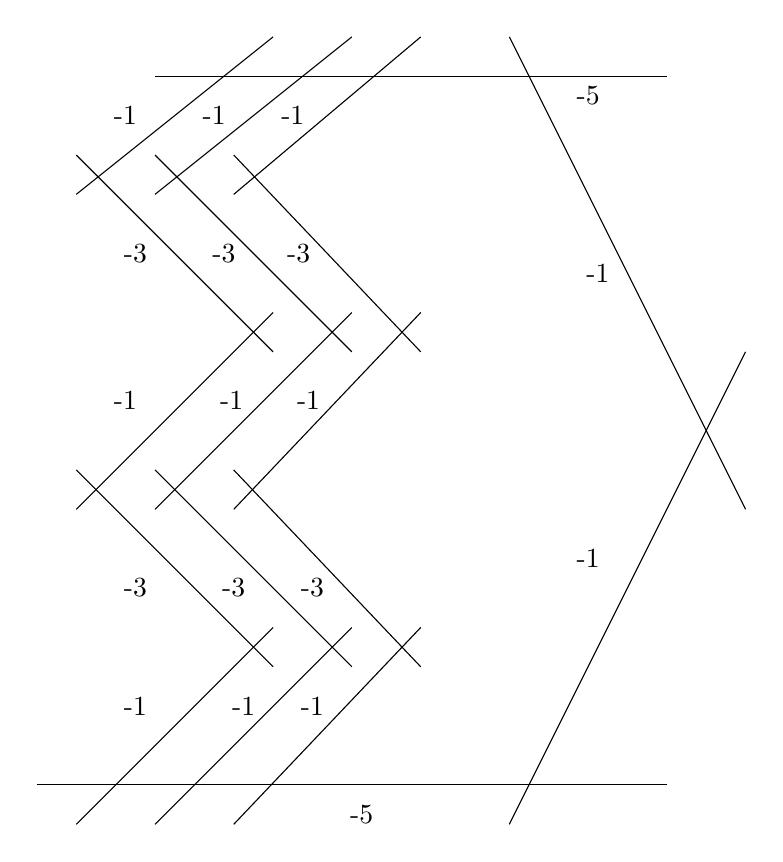
\begin{tikzpicture}[scale = 0.5]
	\begin{pgfonlayer}{nodelayer}
		\node [style=none] (0) at (-3, 3) {};
		\node [style=none] (1) at (10, 3) {};
		\node [style=none] (4) at (2, 4) {};
		\node [style=none] (5) at (-3, 0) {};
		\node [style=none] (6) at (3.75, 4) {};
		\node [style=none] (7) at (-1, 0) {};
		\node [style=none] (8) at (12, -8) {};
		\node [style=none] (9) at (6, 4) {};
		\node [style=none] (10) at (0, 4) {};
		\node [style=none] (11) at (-5, 0) {};
		\node [style=none] (12) at (-5, 1) {};
		\node [style=none] (13) at (0, -3) {};
		\node [style=none] (14) at (-3, 1) {};
		\node [style=none] (15) at (2, -3) {};
		\node [style=none] (16) at (-1, 1) {};
		\node [style=none] (17) at (3.75, -3) {};
		\node [style=none] (20) at (0, -4) {};
		\node [style=none] (21) at (2, -4) {};
		\node [style=none] (22) at (3.75, -4) {};
		\node [style=none] (23) at (-5, -7) {};
		\node [style=none] (24) at (-3, -7) {};
		\node [style=none] (25) at (-1, -7) {};
		\node [style=none] (26) at (-5, -8) {};
		\node [style=none] (27) at (-3, -8) {};
		\node [style=none] (28) at (-1, -8) {};
		\node [style=none] (29) at (-3.75, 2) {-1};
		\node [style=none] (30) at (-1.5, 2) {-1};
		\node [style=none] (31) at (0.5, 2) {-1};
		\node [style=none] (32) at (-3.5, -1.5) {-3};
		\node [style=none] (33) at (-1.25, -1.5) {-3};
		\node [style=none] (34) at (0.65, -1.5) {-3};
		\node [style=none] (35) at (-3.75, -5.25) {-1};
		\node [style=none] (36) at (-1.05, -5.25) {-1};
		\node [style=none] (37) at (0.9, -5.25) {-1};
		\node [style=none] (38) at (2.25, -5.5) {};
		\node [style=none] (39) at (0, -11) {};
		\node [style=none] (40) at (2, -11) {};
		\node [style=none] (41) at (3.75, -11) {};
		\node [style=none] (42) at (0, -12) {};
		\node [style=none] (43) at (2, -12) {};
		\node [style=none] (44) at (3.75, -12) {};
		\node [style=none] (45) at (-6, -15) {};
		\node [style=none] (46) at (-3, -15) {};
		\node [style=none] (47) at (-1, -15) {};
		\node [style=none] (48) at (-5, -16) {};
		\node [style=none] (49) at (-3, -16) {};
		\node [style=none] (50) at (-1, -16) {};
		\node [style=none] (51) at (-3.5, -10) {-3};
		\node [style=none] (52) at (-1, -10) {-3};
		\node [style=none] (53) at (1, -10) {-3};
		\node [style=none] (54) at (-3.5, -13) {-1};
		\node [style=none] (55) at (-0.75, -13) {-1};
		\node [style=none] (56) at (1, -13) {-1};
		\node [style=none] (57) at (10, -15) {};
		\node [style=none] (58) at (12, -4) {};
		\node [style=none] (59) at (6, -16) {};
		\node [style=none] (60) at (8.25, -2) {-1};
		\node [style=none] (61) at (8, -9.25) {-1};
		\node [style=none] (62) at (2.25, -15.75) {-5};
		\node [style=none] (63) at (8, 2.5) {-5};
	\end{pgfonlayer}
	\begin{pgfonlayer}{edgelayer}
		\draw (11.center) to (10.center);
		\draw (5.center) to (4.center);
		\draw (7.center) to (6.center);
		\draw (12.center) to (20.center);
		\draw (14.center) to (21.center);
		\draw (16.center) to (22.center);
		\draw (0.center) to (1.center);
		\draw (26.center) to (13.center);
		\draw (27.center) to (15.center);
		\draw (28.center) to (17.center);
		\draw (23.center) to (42.center);
		\draw (24.center) to (43.center);
		\draw (25.center) to (44.center);
		\draw (39.center) to (48.center);
		\draw (49.center) to (40.center);
		\draw (41.center) to (50.center);
		\draw (45.center) to (57.center);
		\draw (9.center) to (8.center);
		\draw (58.center) to (59.center);
	\end{pgfonlayer}
\end{tikzpicture}
\]
\begin{lem}
This surface does not admit a toric degeneration.
\end{lem}
\begin{proof}
Given a Looijenga surface $X$,
 in the sense of \ref{Something chapter 2}, %Change this to make it make sense!
 and a curve $C$ in the boundary. Let $C_1,$ $\dots, $ $C_n$ be the $-1$-curves intersecting $C$. Then at most two of these $-1$-curves intersect curves with self intersection less than $-1$, as they would have to be in the boundary which is a cycle. The $-5$ curves in the above picture clearly do not satisfy this constraint, hence this surface does not admit a well defined boundary.
\end{proof}
However this surface has six $\frac{1}{3}(1,1)$ singularities and two $\frac{1}{5}(1,1)$ singularities and the following invariants
\begin{itemize}
\item $-K_X^2 = \frac{2}{5}$
\item $h^0(-K_X) = 1$
\end{itemize}
This is a complexity one surface, and the calculations can be done via polyhedral divisors as set out in \cite{Polarised polyhedral divisors}. 
Alternatively we know this is constructed by 13 blowups of a Hirzebruch surface and then 8 subsequent contractions. This gives $-K_X^2 = 8 - 13 + 6 v_{\frac{1}{3}(1,1)} + 2 v_{\frac{1}{5}(1,1)}$ where the $v_i$ are correction terms in orbifold Riemann-Roch \cite{Young}. We calculate them to be $v_{\frac{1}{3}(1,1)}  = \frac{5}{3}$ and $v_{\frac{1}{5}(1,1)}  = \frac{1}{5}$. This gives $-K_X^2 = \frac{2}{5}$. We see once again via \cite{Young} that we can calculate $h^0(-K_X)$ from this and get $h^0(-K_X) = 1$.


We can construct this surface as a toric complete intersection via cox rings \cite{HausenCox} and we see that it lies as a complete intersection in the toric variety given by the GIT quotient
\[
\begin{blockarray}{cc cc cc cc cc c}
	T_1 & T_2 & T_3 & T_4 & T_5 & T_6 & T_7 & T_8 & T_9 & T_{10} & T_{11} \\[4pt]
      \begin{block}{(cc cc cc cc cc c)}
	1&-2&3&0&0&0&0&0&0&0&0 \\ 
	0&3&-6&-2&1&0&0&0&0&0&0 \\
	0&2&-4&-1&0&1&0&0&0&0&0 \\
	0&3&-6&0&0&0&-2&1&0&0&0 \\ 
	0&2&-4&0&0&0&-1&0&1&0&0 \\
	0&-3&7&1&0&0&1&0&0&1&0 \\
	0&1&-2&0&0&0&0&0&0&-1&1 \\
      \end{block}
\end{blockarray}
\]
with the equations 
\[
T_1 T_2^2 T_3 + T_4 T_5^2 T_6 + T_7 T_8^2 T_9 = 
T_1 T_2^2 T_3 + T_4 T_5^2 T_6  + \lambda T_{10} T_{11} = 0
\]
To do this we note that this surface has polyhedral divisor, as introduced in Chapter 4
\[ 
\left[ 0, \, \frac{3}{2}, \, 3 \right] \otimes P_1 + \left[ 0, \, \frac{3}{2}, \, 3 \right] \otimes P_2 + \left[ 0, \, \frac{3}{2}, \, 3 \right] \otimes P_3 + \left[ -5, \, -4 \right] \otimes P_4
\]
Where $\lambda$ is a deformation parameter. This gives us equations for the surface, to obtain the weights we calculate the action of the picard torus via taking the smith normal form of the matrix representing relations on the class group. We do not provide this calculation as it is largely disjoint from the rest of this Thesis. We note that there are also surfaces which admit a toric degeneration with the same numerics.


\chapter{Complexity One log Del Pezzo Surfaces}

\section{Introduction}

All varieties we consider are normal and projective. Here we give an algorithm to classify Log Del Pezzos admitting a $\mathbb{C}^\times$ action with only log terminal singularities. A variety $X$ of dimension $n$ which admits a torus action of dimension $n-k$ is referred to as complexity $k$. Here complexity 0 is the study of purely toric varieties, and complexity $n$ is the study of varities with no possible torus action. This provides essentailly a way of grading the difficulty of your problem. Significant progress has been made on this problem before: S\"{u}ss \cite{Suss} classifies log del Pezzo surfaces admitting said action with Picard rank one and index less than 3. Huggenberger \cite{Huggenberger} classifies the anticanonical complex of the Cox ring of log del Pezzo surfaces with index 1, this classification was later finished by Ilten, Mishna and Trainor \cite{IMT} with a view towards higher dimension. This was achieved by looking at polarised complexity one log del Pezzo surfaces. We will show their work fits into our algorithm. 
\\
\\
\section{Polyhedral divisors}
Recall that a toric variety is a  normal variety of dimension $n$ containing a dense torus $\C{n}$ with the natural action extending to the variety, there is a one to one correspondence between these varieties and fans inside a lattice $N \cong \mathbb{Z}^n$ upto GL$_2(\mathbb{Z})$, \cite{Cox}.
Altman et.al \cite{Altmann} establish a similar correspondence for varieties with $T = \C{{ n-k}}$ actions where $k \leq n$. We say that this is a torus action of complexity $k$. They introduce the notion of a polyhedral divisor to recover some of the geometry that a fan encodes in the toric case. In general this applies for any complexity, however the behaviour is easiest to describe in the toric case, then complexity one until you reach the full general case.


Given $X$, a variety with dimension $n$ admitting of the torus $ T = (\mathbb{C}^*)^{n-1}$ action, we can take a Chow quotient $Y$ of $X$ by $T$, essentially a GIT quotient followed by normalisation.  We see that $Y$ will be a variety of dimension $k$, we can resolve this map to $\tilde{X}$ getting the following diagram

\[
\begin{tikzcd}
X \arrow[rd, dotted] & \tilde{X} \arrow[l] \arrow[d]\\
& Y
\end{tikzcd}
\]

Here $Y \cong C$ is a normal curve. In this thesis we will primarily be interested in the case where $C \cong \mathbb{P}^1$. We start by introducing the notion of a tail cone of a given polyhedral cone. This is given $F$ a polyhedral subdivision such that the tail cone $\delta$ is the set of $v \in N$ such that $F_i$ is invariant under the translation, so $\delta = \{ v |\, v(F) subset F \}$.
\begin{dfn}
Let $C$ be a nonsingular curve then we define a polyhedral divisor to be the pair $(\mathcal{D} = \sum_{i = 1}^k F_i \otimes P_i$, $\delta)$ where
\begin{itemize}
\item $P_i \in C$ are divisors on $C$ 
\item $F_i$ is a polyhedron contained in $N_\mathbb{Q} \cong \mathbb{Q}^{n-1}$ and all $F_i$ have tail cone $\delta \subset N$.  We allow the cone $F_i$ to be $\varnothing$.
\end{itemize}
Given an element $v \in M$, the dual lattice of $N$, and the polyhedral divisor $\mathcal{D}$ we define
\[
\mathcal{D}(v) = \sum \min_{u \in F_i} \langle u, v \rangle P_i
\]
This is defined as a divisor on the following curve
\[
Y_\mathcal{D} = C - \{P_j\}_{j \text{ where } F_j = \varnothing}
\]
\end{dfn}

This defines a divisor on a subset of $C$. We insist that $\mathcal{D}$ satisfies the following conditions:
\begin{enumerate} 
\item $\mathcal{D}(u)$ is Cartier for all $u \in \delta^\vee $
\item $\mathcal{D}(u)$ is semiample for all $u \in \delta^\vee$
\item $\mathcal{D}(u)$ is big for all $u$ in the relative interior of $\delta^\vee$
\end{enumerate}
This is to ensure that it gives an $n$-dimensional variety, and to ensure that it is separated \cite{PS}.


We can now calculate the associated affine varieties $X$ and $\tilde{X}$ by taking respectively Spec/ RelSpec${_C}$ of the graded ring
\[
\bigoplus_{v \in \delta^\vee} \mathcal{O}_{Y_\mathcal{D}} ( \mathcal{D}(v))
\]
This gives us an affine variety with $T = \text{Spec } \mathbb{C}[M]$ acting by torus action. Analogous to the toric case, if $F_i \subset F_j$ is a face then we have
\[
\bigoplus_{v \in \delta^\vee} \mathcal{O}_{Y_\mathcal{D}}( \mathcal{D}_{F_j}(v)) \subset \bigoplus_{v \in \delta^\vee} \mathcal{O}_{Y_\mathcal{D}}( \mathcal{D}_{F_i}(v)) 
\]
This corresponds to an inclusion of schemes. We make the following comment that taking a divisor 
\[ 
\mathcal{D} = \sum_{i = 1}^n F_i \otimes P_i + \varnothing \otimes P_{n+1}
\]
is the same as taking the divisors 
\[
\mathcal{D}_i = F_i \otimes P_i  + \sum_{j=1, \, j \neq i} \varnothing \otimes P_j
\]
and then glueing these affine varieties together along the affine patch defined by $C-P_i - P_j$ for all $P_i$, $P_j$. We say that if the tail cone of a polyhedral divisor $\mathcal{D}$ is non zero and there is no point $P$ such that $\mathcal{D}|_P = \varnothing$ then $\mathcal{D}$ is marked. The variety $\widetilde{X}$ is defined to be the variety such that the cone is not marked.


We now introduce the notion of a polyhedral fan. Consider a collection of polyhedral divisors $\mathcal{S} = \{ \mathcal{D}_i \}$ such that the tail cones form a fan in the sense of toric geometry, we call this the tail fan. Given $\mathcal{S} \ni \mathcal{D}_i = \sum \sigma^i_j \otimes P_j$ then  we can make the divisor $\mathcal{D} = \sum \tau_j \otimes P_j$ where $\tau_j$ a face of each cone corresponding to a face of the tail cone. If $\mathcal{D} \in \mathcal{S}$ for all possible faces of all the tail cone, then this is a polyhedral fan. As this is stated above this makes no mention of how this behaves with respect to a divisor $\mathcal{D} = \sum \sigma_i \otimes P_i + \varnothing \otimes P$. 
To do this we add that if given a face of the tail fan $\delta$ there is associated polyhedral divisor $\mathcal{D} = \sum \sigma_i \otimes P_i$ with $\delta$ as its tail cone. We then insist that if a cone in the tail fan is not marked then every face of the cone is also not marked. If the collection $\mathcal{S}$ satisfies these conditions then we call it a polyhedral fan.


Given a complexity one projective variety $X$ over a curve $C$ this corresponds to a polyhedral fan with the tail fan spanning $N$. Analaously to the case in cones, the variety $\widetilde{X}$ is defined to be the complexity one variety with the same tail fan and polyhedral divisors however every cone is not marked. The action of the $(\mb{C}^\times)^{n-1}$ on $\widetilde{X}$ corresponds to a fibration over $C$ with general fiber $X_t$ equal to the toric variety defined by the tail fan. The degenerate fibers are then described by the polyhedral fans. 



In the case of surfaces of complexity one we often use the notation of fansy divisors as set out in \cite{Suss}. This follows the key notion that in the case of $n=2$ and $k=1$ we have that every tail fan is either $0$, $\mathbb{Z}_{\geq 0 }$ or $\mathbb{Z}_{\leq 0}$ We have $n$ subdivisions of $N \cong \mathbb{Z}$, these should be viewed as the polyhedral divisors over these $n$ points. Note that if we have a closed interval in any of subdivisions this will have tail fan zero and these give rise to a cyclic quotient singularity, with a nice torus quotient, i.e the map to $\tilde{X}$ is a contraction to a point. It is the intervals $[a_1, \infty )$ which provide difficulty, if as polyhedral divisors these are all of the form 
\[
\mathcal{D}_i = [a_i, \infty) \otimes P_i + \sum_{\substack{j = 1 \\ j \neq i}}^n \varnothing \otimes P_j
\]
\textbf{Change this paragraph}
Then this gives rise to a nice quotient map down base curve with respect to the torus action, i.e  the map to $\tilde{X}$ is a local isomorphism. If this is not the case however, then we are left with a bad quotient. In the surface case, there are the only two cases that can occur. In the language of fansy divisors we say if we mean the latter case we denote it with $\mathbb{Q}^+$, if we mean the other the earlier case, we do no denote it at all. In this way fansy divisor uniquely specify polyhedral fans.
\\
\\
\section{Examples}

\begin{ex}[\label{ToricDowngrade}]
The first is the polyhedral divisor given by the unmarked polyhedral divisor $[0, 1] \otimes P_0$ over $Y = \mb{P}^1$. 
The tail cone $\delta$ is equal to $0$. We will show how we can construct from this an affine variety $X$. We denote the polyhedral divisor by $\mathcal{D}$. So the dual of the tail cone $\hat{\delta}$ is the lattice $M$ itself. Given an element $ m >0$ of $M$ we have $\mathcal{D}(m) = -mP_0$ as the minimum value is obtained on $-1$. If $m <0$ we get $\mathcal{D}(m) = mP_0$  as the minimum is attained on 1. Finally if $n=0$ we get $\mathcal{D}(m) = 0$ as a divisor on $\mathbb{A}^1$ as the function is 0 everywhere. 


Hence we have the $M$ graded ring
\[
\bigoplus_{m \in M} \mathcal{O}_{\mathbb{A}^1}(-|m|P)
\]
In degree 0 the ring is generated by the constant function on $\mb{A}^1$ which we denote $x$ and the function $y$ which is zero at the origin. We note that the function $1$ in degree 0 is the multiplicative identity of our ring. In degree one every element is of the form $f ( a_0 x + a_1 y + a_2 y^2 + \dots  a_n y^n)$, here $f$ is the same function on $\mb{A}^1$ as $y$ but now in degree 1. Every element of degree $m>0$ is of the form $f^m ( a_0 x + a_1 y + a_2 y^2 + \dots  a_n y^n)$. Hence this ring is generated in degree 1. The calculation on the ring graded in negative degree is exactly the same, except with a function $g$.  We note that $fg = y^2$ as $f$ and $g$ are both equal to $y$ as functions on $\mb{A}^1$. We finally discuss the function $x$. Given a function $F \in \mb{C}(X)$, then $F = \sum F_i \chi^{m_i}$, here the $F_i$ are functions on the curve $Y$ and $\chi^{m_i}$ are monomials in the lattice $M$. By construction the function $x = \mathbbm{1}_{Y} \, \chi^0$, hence $x$ is the constant function on the variety. Hence we get the ring $\mathbb{C}[f,  \, g, \, y]/ (fg=y^2)$, so an $A_1$ singularity.
\end{ex}

We can more generally describe what occurs with polyhedral divisors of the form $[\frac{a}{b}, \, \frac{c}{d}] \otimes P_0$ with $\frac{a}{b} < \frac{c}{d}$. We note that the tail cone $\delta$ is always 0 and so the dual tail cone is all of $M$. From the definitions we get the ring $R = \bigoplus_{m \in M} R_m \chi^m$ where

\[
R_m = 
\begin{cases}
\mathcal{O}_{\mb{A}_z^1} ( \frac{ma}{b}P) & \text{if } m \geq 0,  \vspace{0.2cm} \\
\mathcal{O}_{\mb{A}_z^1} ( \frac{mc}{d}P) & \text{if } m \leq 0.
\end{cases}
\]

We can associate the monomial $z^u \chi^v$ with the lattice point $(u,v)$ inside a two dimensional monomial lattice. This gives rise to a cone $\sigma$. The set of monomials with poles of order at worst $\frac{a}{b}$ gives rise to the vector $(a, -b)$. Similarly the other side of the graded ring gives rise to the vector $(-c, d)$. These are boundary rays of $\sigma$, this means that as toric variety they can be described as the cone $(a,b)$, $(c,d)$ inside the lattice $N \cong \mathbb{Z}^2$ with torus action corresponding to $(1,0)$.  Hence we get a toric variety of the form $\frac{1}{r}(\alpha, \, \beta)$ where $r = bc-ad$ and $\alpha$ and $\beta$ are generators of the kernel of the matrix $M$ modulo $r$ where
\[
M =  \begin{pmatrix} c & a \\ d & b \end{pmatrix} 
\]

% Expand this to fans, mention this 


\begin{ex}\rm
We now show how this behaves in the case of a divisor with tail cone $\delta = [0, \, \infty)$. Consider the divisor $\mathcal{D} = \left[\frac{1}{2}, \, \infty \right) \otimes P_0 + \left[\frac{1}{2}, \, \infty \right) \otimes P_1 + \left[\frac{-1}{2}, \, \infty \right) \otimes P_2$ over $\mb{P}^1$ with coordinates $x_1, \, x_2$. Here the varieties $X$ and $\widetilde{X}$ are different. To start with, we look at how to construct $X$. For simplicity we assume $P_0 = (1; \, 0)$, $P_1 = (1; \, 1)$ and $P_2 = (0; \, 1)$.

The tail cone is $\delta = [0, \, \infty)$ so $\hat\delta = [0, \, \infty)$. By calculating $\mathcal{D}(m)$ we get the following ring
\[
\bigoplus_{m \in M|_{\geq 0}} \mathcal{O}_{\mb{P}^1} \left( \frac{m}{2} P_0 + \frac{m}{2} P_1 + \frac{-m}{2} P_2 \right)
\]
Once again in degree 0 we get the constant function. In degree one we get no functions. In degree 2 we get 2 functions $\frac{x_2}{x_1} \chi^2 $ and $\frac{x_2}{x_1-x_2} \chi^2$ denote these $u$ and $v$. In degree 3 we get the function $\frac{x_2^2}{x_1(x_1-x_2)} \chi^3 $ denote this by $w$. We then have the relations $w^2 = uv(v-u)$. This gives rise to a $D_4$ singularity.  

To calculate $\widetilde{X}$ we do all these calculations as relative spec. In particular this means we can our above graded ring with the following three graded rings
\[
\bigoplus_{m \in M|_{\geq 0}} \mathcal{O}_{(\mb{P}^1 - P_i - P_j)} \left( \frac{m}{2} P_0 + \frac{m}{2} P_1 + \frac{-m}{2} P_2 \right)
\]
For all choices of $i$ and $j$. We then glue together on the intersection. Calculating in the case $i=1$ and $j =2$. We have
\[
\bigoplus_{m \in M|_{\geq 0}} \mathcal{O}_{(\mb{P}^1 - P_1 - P_2)} \left( \frac{m}{2} P_0 + \frac{m}{2} P_1 + \frac{-m}{2} P_2 \right) \cong \bigoplus_{m \in M|_{\geq 0}} \mathcal{O}_{(\mb{A}^1 - P_1)} (\frac{m}{2}P_0)
\]
This gives us the ring $\mb{C}[x, \frac{1}{x+1}, \frac{1}{x}\chi^2, \chi^1] = \mb{C}[u,v,w,t]/[v(u+1) = 1, \, uw = t^2]$. Hence this is an $A_1$ singularity. The calculations on the other 3 patches are the same, so we have taken the partial resolution of the $D_4$ singularity by extracting the trivalent curve. 
\end{ex}


\begin{ex}\rm
Consider the following polyhedral fan with marking $\mb{Q}^\pm$
\[
\begin{tikzpicture}
	\begin{pgfonlayer}{nodelayer}
		\node [style=none] (0) at (-7, 4) {};
		\node [style=none] (1) at (-7, 4.25) {};
		\node [style=none] (2) at (-7, 3.75) {};
		\node [style=none] (3) at (-3, 4) {};
		\node [style=none] (4) at (-3, 4.25) {};
		\node [style=none] (5) at (-3, 3.75) {};
		\node [style=none] (6) at (0, 4) {};
		\node [style=none] (7) at (-10, 4) {};
		\node [style=none] (14) at (0, 2) {};
		\node [style=none] (15) at (-10, 2) {};
		\node [style=none] (16) at (-4, 1.75) {};
		\node [style=none] (17) at (-4, 2.25) {};
		\node [style=none] (18) at (-10, 0) {};
		\node [style=none] (19) at (-6, 0.25) {};
		\node [style=none] (20) at (-6, -0.25) {};
		\node [style=none] (21) at (0, 0) {};
		\node [style=none] (22) at (-7, 3.25) {};
		\node [style=none] (23) at (-7, 3.25) {-1};
		\node [style=none] (24) at (-3, 3.25) {1};
		\node [style=none] (25) at (-4, 1.25) {};
		\node [style=none] (26) at (-4, 1.25) {$\frac{1}{2}$};
		\node [style=none] (27) at (-6, -0.75) {};
		\node [style=none] (28) at (-6, -0.75) {$-\frac{1}{2}$};
		\node [style=none] (29) at (-10, -2) {};
		\node [style=none] (30) at (0, -2) {};
		\node [style=none] (31) at (-5, -2) {};
		\node [style=none] (32) at (-5, -2.75) {};
		\node [style=none] (33) at (-5, -2.75) {0};
		\node [style=none] (34) at (2, 5) {};
		\node [style=none] (35) at (2, -3) {};
		\node [style=none] (36) at (1.5, 1) {$\mathbb{P}^1$};
		\node [style=none] (37) at (2.5, -2) {};
		\node [style=none] (38) at (2.5, -2) {$P_{\text{gen}}$};
		\node [style=none] (39) at (2.5, 0) {$P_\infty$};
		\node [style=none] (40) at (2.5, 2) {};
		\node [style=none] (41) at (2.5, 2) {$P_1$};
		\node [style=none] (42) at (2.5, 4) {$P_0$};
		\node [style=none] (43) at (-5, -2.25) {};
		\node [style=none] (44) at (-5, -1.75) {};
	\end{pgfonlayer}
	\begin{pgfonlayer}{edgelayer}
		\draw (1.center) to (2.center);
		\draw (4.center) to (5.center);
		\draw (17.center) to (16.center);
		\draw (19.center) to (20.center);
		\draw [style=new edge style 1] (21.center) to (18.center);
		\draw [style=new edge style 1] (15.center) to (14.center);
		\draw [style=new edge style 1] (7.center) to (6.center);
		\draw [style=new edge style 1] (29.center) to (30.center);
		\draw [style=new edge style 1] (34.center) to (35.center);
		\draw (43.center) to (44.center);
	\end{pgfonlayer}
\end{tikzpicture}
\]
We now go through each polyhedral divisor and calculate the associated rings. 
There are three polyhedral divisors contained inside this polyhedral fan which are one dimensional cones. There are three polyhedral divisors which correspond to two dimensional cones. 

\begin{enumerate}[label =\alph*)]
\item The unmarked polyhedron $[-1, \, 1]$
\item The marked cone $1\otimes P_0 + \frac{1}{2} \otimes P_1 + \frac{-1}{2} \otimes P_\infty$ with tail cone $[0,\, \infty)$.
\item The marked cone $-1\otimes P_0 + \frac{1}{2} \otimes P_1 + \frac{-1}{2} \otimes P_\infty$ with tail cone $(-\infty, \, 0]$.
\end{enumerate}

In case $a$ the tail cone $\delta$ is equal to $0$. We denote the polyhedral divisor by $\mathcal{D}$. So the dual of the tail cone $\hat{\delta}$ is the lattice $M$ itself. Given an element $ m >0$ of $M$ we have $\mathcal{D}(m) = -mP_0$. If $m <0$ we get $\mathcal{D}(m) = mP_0$ and if $n=0$ we get $\mathcal{D}(m) = 0$ as a divisor on $\mathbb{A}^1$. 

Hence we have the $M$ graded ring
\[
\bigoplus_{m \in M} \mathcal{O}_{\mathbb{A}^1}(-|m|P)
\]
In degree 0 the ring is generated by the constant function $x$ and the function $y$ which is zero at the origin. We note that the function $1$ in degree 0 is the multiplicative identity of our ring. In degree one every element is of the form $f ( a_0 x + a_1 y + a_2 y^2 + \dots  a_n y^n)$, here $f$ is the same function as $y$ but now in degree 1. Every element of degree $m>0$ is of the form $f^m ( a_0 x + a_1 y + a_2 y^2 + \dots  a_n y^n)$. Hence this is generated in degree 1. The calculation on the ring graded in negative degree is exactly the same.  Hence we get the ring $\mathbb{C}[f,  \, g, \, y]/ (fg=y^2)$, so an $A_1$ singularity.


In case $a$ the tail cone $\delta$ is equal to $[0 ,  \, \infty)$. We denote the polyhedral divisor by $\mathcal{D}$. So the dual of the tail cone $\hat{\delta}$ is $[0 ,  \, \infty) \subset M$. Given an element $ m \geq 0$ of $M$ we have $\mathcal{D}(m) = mP_0 +\frac{m}{2} P_1 + \frac{-m}{2}P_2$. 

Hence we have the $M$ graded ring
\[
\bigoplus_{m \in M|_{\geq 0}} \mathcal{O}_{\mathbb{P}^1} \left(mP_0 +\frac{m}{2} P_1 + \frac{-m}{2}P_2 \right) \cong \bigoplus_{m \in M|_{\geq 0}} \mathcal{O}_{\mathbb{P}^1} \left(\frac{m}{2} P_1 + \frac{m}{2}P_2 \right)
\]
Here the isomorphism follows via linear equivalence of divisors on $\mathbb{P}^1$.

In degree 0 we just get the constant function. In degree 1, once again it is only the constant function, denoted this by $x$. In degree 2 we have the function with a pole at $P_1$ and a zero at $P_2$, denote this by $f$ and the function $g = \frac{1}{f}$. This generates the ring hence we have $\mathbb{C}[x, \, f, \, g]/(fg = x^4)$, so an $A_3$ singularity.


Case $c$ is exactly the same as case $b$ but with the grading negative instead of positive. So it is also an $A_3$ singularity.


We finish by discussing the unmarked polyhedral divisors

\begin{enumerate}[label =\Alph*)]
\item The unmarked cone $-1 \otimes P_0$
\item The unmarked cone $1 \otimes P_0$
\item The unmarked cone $\frac{1}{2} \otimes P_1$
\item The unmarked cone $-\frac{1}{2} \otimes P_2$
\end{enumerate}

In all case the tail cone $\delta$ is equal to 0. In case $A$ have the following ring graded by $M$

\[
\bigoplus_{m \in M} \mathcal{O}_{\mathbb{A}^1}(-mP) \cong \mathbb{C}[x,\, y, \, z]/(yz = 1)
\]
Here $x$ is of degree 0, $y$ is of degree 1 and $z$ is of degree $-1$. Case $B$ is symmetrical to case $A$. 

Cases $C$ and $D$ are also symmetrical, and give rise to the rings $\mathbb{C}[x, y_1, y_2, z_1, z_2]$ with relations induced by the second veronese embedding of $C[x, \, y, \, z]/(yz = 1)$. 


We explicitly describe the maps $1)$ and $2)$. To see map $1)$ the base is 
\[
\bigoplus_{m \in M|_{\leq 0}} \mathcal{O}_{\mathbb{P}^1} \left(-mP_0 +\frac{-m}{2} P_1 + \frac{m}{2}P_2 \right) 
\]
and the image is 
\[
\bigoplus_{m \in M} \mathcal{O}_{\mathbb{A}^1}(-mP_0)
\]
There is clearly an inclusion of rings on each level of the negative grading, and this induces the entire map
\end{ex}

We also provide a quick example of when a polyhedral divisor is unmarked but has unmarked subcones cones as the boundary. 

\begin{ex}\rm
Let $N$ be $\mb{Q}^2$. Consider the polyhedral divisor defined by $\delta \otimes P_0 + ((1, 1) + \delta) \otimes P_1$ over $\mathbb{P}^1$ where $\delta = \langle (1,0) , \, (0, 1) \rangle$. We now insist that two dimensional cone is marked. However if we pick a ray of the tail fan, and calculate the dual we see that this does not satisfy of being semiample on the boundary, if the base curve was non affine.

Upon calculation of the affine ring this can be seen as a toric downgrade of the Atiyah flop, with the quotient corresponding to one of the two natural maps to $\mathbb{P}^1$. To see the two flops the first is by unmarking the two dimensional cone and the other is given by the same polyhedral coefficients but now the tail cone is a tail fan with the ray $(1,1)$ bisecting it. This corresponds to only one of the resolutions resolving the quotient down to the $\mathbb{P}^1$.
\end{ex}

\begin{comment}
\begin{dfn}
A fansy divisor a smooth curve $C$ is a collection of $n$ subdivison of $\mathbb{Q}$ with markings $\mathbb{Q}^+$, $\mathbb{Q}^-$, $\mathbb{Q}^\pm$ or no markings at all. 
\end{dfn}
This is equivalent to a polyhedral divisor provided the the assumptions of \ref{Tech} are satisfied.


This defines a complexity one surface. 
\end{comment}

In toric varieties full dimensional cones give rise to torus fixed point. Analogously, the same way for varieties of higher complexity every full dimensional subdivision of the plane gives rise to a toric fixed point. In the case of surfaces these fixed points can be classified giving rise to three cases
\begin{itemize}
\item $\bold{Elliptic}$ - Around the fixed point in local coordinates, the torus behaves on all coordinates with positive or negative degree. These points are isolated.
\item $\bold{Parabolic}$ - These always arise as blowups of elliptic points, these occur when in local coordinates, one of the coordinates is acted trivially upon by the torus. These points lie on a section of the map to $Y$
\item $\bold{Hyperbolic}$ - These are where the the local coordinates are acted in positive and negative degree.
\end{itemize}
It is easy to see that Hyperbolic points correspond to a subdivision with $\delta = 0$, Parabolic correspond to an unmarked edge going to infinity and Elliptic to a marked point going to infinity.
\section{Divisors in complexity one}

We now limit ourselves strictly to complexity one, and the chow quotient $Y$ will now be $\mathbb{P}^1$. In the torus setting we know that divisors correspond to rays of the associated fan. Almost exactly the same is true in complexity one: divisors  occur as torus invariant divisor, these correspond the codimension 1 polyhedral divisors or they are premimages of the $\mathbb{P}^1$. These correspond to a polyhedral divisor $\mathcal{D}$  going of to infinity in a direction, with dim$(\delta) = \infty$ which forall $P \in \mathbb{P}^1$ we do not have $\mathcal{D}  |_P = \varnothing$. Note that this also holds for higer dimensions, with a little bit of extra work. From this it is easy to derive the following theorem
\\
\begin{thm}[\cite{PS}]
The Picard rank of a complexity one surface defined by a polyhedral fan $\mathcal{S}$ is 
\[
\rho_X =  \text{ \# Number of parabolic lines } + \sum_{P \in Y} (\# \mathcal{S}_P^{(0)} - 1) 
\]
\end{thm}
where $n$ is the dimension and $\# \mathcal{S}_P^{(0)}$ is the number of points on this slice of the fan. Similar statements can be made in dimension $n$ where the parabolic lines are replaced by x-rays. In a similar style to this we can classify Cartier divisors, we here make no pretense at proof or justification. 
\begin{dfn}
A divisorial support function $h$ on a divisorial fan $\mathcal{S}$ is a piecewise linear function on each component of the fan such that

\begin{itemize}
\item On every polyhedron $\Delta \in \mathcal{S}_{P_i}$ it is a linear function
\item $h$ is continuous
\item at all points $h$ has integer slope and integer translation
\item if $\mathcal{D}_1$ and $\mathcal{D}_2$ have the same tail cone, then the linear part of $h$ restricted to them is equal
\end{itemize}
\end{dfn}
We call a support function principal if it is of the form $h(v) = \langle u, v \rangle + D$, this corresponds to a principal Cartier divisor. We call a support function Cartier, if on every component with complete locus the support function is principal. In the case of Fansy divisors, this just correspond to the edge with a marking. We denote $h$ restricted to a component by $h_P$.  We refer to a piecewise linear function with rational slope and rational translation as a $\mathbb{Q}$ support function.
\begin{thm}[\cite{PS}]
Let $X$ be the variety associated with the divisorial fan $\mathcal{S}$. There exists a one to correspondence between support functions support function quotiented by principal support functions and Cartier divisors on the complexity one variety. In addition there exists 
a one to correspondence between $\mathbb{Q}$ support functions support function quotiented by principal support functions and $\mathbb{Q}$ Cartier divisors on the complexity one variety

\end{thm}
Using the above languages we represent the canonical divisor as a Weil divisor, it has the following form
\begin{thm}[\cite{PS}]
The canonical divisor of a complexity one surface can be represented in the following form
\[
K_X = \sum_{(P, v)} ( \mu (v) K_Y (P) + \mu (v) - 1) \cdot D_{(P,v)} - \sum_\rho D_\rho
\]
\end{thm}
Here $K_Y(P)$ is the degree of $K_Y$ at $P$, and $\mu (v)$ is the smallest value $k$ such that $k \cdot v \in \mathbb{N}$.  While I have not stated the conditions for linear equivalence these can be seen in \cite{PS}, and using these you can show that it does not depend on the choice of representative of $K_Y$. Note that given the singularities and varieties we are working with we know that our $K_X$ will be $\mathbb{Q}$-Cartier. The fano index is clear and easy to derive from the singularities we have, so all that remains is to check on the conditions for a complexity one divisor to be ample.

\begin{thm}[\cite{PS}]
A suppport function $h$ is ample iff for all $P$ we have $h_P$ is strictly concave, and for all polyhedral divisors $\mathcal{D}$ defined on an affine curve we have
\[
- \sum_{P \in \mathbb{P}^1} h_P |_\mathcal{D} (0) \in \text{Weil}_\mathbb{Q} (Y)
\]
 is an ample $\mathbb{Q}$ Cartier divisor.
\end{thm}
Note that in reality $h_P |_\mathcal{D}$ may not be defined at $0$ but we can extend the affine function to $0$. We finish this recap on divisors by describing the Weil divisor corresponding to a Cartier divisor
\begin{thm}[\cite{PS}]
Let $h = \sum_P h_P$ be a Cartier divisor on $\mathcal{S}$ then the corresponding Weil divisor is 
\[
- \sum_\rho h_t ( n_\rho) D_\rho - \sum_{(P, v)} \mu(v) h_P(v) D_{(P,v)}
\]
\end{thm}
Here $n_\rho$ is the generator of the ray inside the tail fan and $\mu(v)$ is as before. Note that is easy to see why we need this $\mu$ function. If you start with a closed subinterval $[a, b]$ and try to work out what the corresponding affine variety is, we see that it just the toric variety defined by the cone $(a,1), \, (b,1)$, and then all you calculations can be done in the realm of toric varieties, however there you use the generator of your rays in the lattice, so you need the $\mu$ function.
\\
\\
We use the above note to easily calulate the minimal resolution of a complexity one surface. Note that we can split this across affine charts, in the first case if we have the affine chart corresponding to the polyhedral divisor $[a,b]$ then using the above point we can can calculate this by the toric methods. In case two where we have a non marked edge going to infinity, we can split this into affine charts $[a_i, \infty)$ this is also a toric chart corresponding to the cone $(a,1), \, (1,0)$, so once again the resolution is toric. The final case is with a marked edge, however we can take a weighted blowup to resolve the ellitic point, then resolve the resulting singularities by the above methods. To calculate the intersection numbers on the resolution you can either use \cite[Tim], \cite{PS} or you can note that the only part that is not toric is the parbolic line, this is defined by glueing together charts coming from $[a_i', \infty)$, here by smootheness $a_i' \in \mathbb{Z}$, this is isomorphic to the charts defined by $[\sum(a_i'), \infty)$ at $P_1$ and $[0, \infty)$ for all other $P_i$. Hence we see that the parabolic line is define torically as the fan  
$(\sum(a_i'), 1), \, (1, 0), \,(0, -1)$ from this an easy derivation of the intersection number follows.


\section{Algorithm}
We begin with the following lemma:
\begin{lem}{\cite{Suss}}
Let $S$ be a non cyclic complexity one log terminal surface singularity. Then $S$ has, upto isomorphism, a fan over $\mathbb{P}^1$ with coefficients
\[
\left[\frac{p_1}{q_1}, \infty \right) \otimes P_1 + \left[ \frac{p_2}{q_2}, \infty \right) \otimes P_2 + \left[ \frac{p_3}{q_3}, \infty \right) \otimes P_3
\]
with $(q_1, q_2, q_3)$ satisfying $\sum(1 - \frac{1}{q_i}) < 2$.
\end{lem}
\begin{proof}
See \cite{Suss}
\end{proof}
In particular this means the only possible denominators are $(2,2,m),$ $(2,3,3)$, $(2,3,4)$ and $(2,3,5)$, we call these of type $D_n$, $E_6$, $E_7$ and $E_8$ respectively. 

We now state the following  lemma
\begin{lem}{\label{trivalent}}
Let $S$ be a log terminal surface singularity of Gorenstein index $l$. Let $E$ be an exceptional curve in the minimal resolution. Then $E^2 \geq -2l$ if it is not a trivalent curve and $E^2 \geq -3l$ if it is trivalent.
\end{lem}
\begin{proof}
Via the classification of log terminal singularities \cite{Br} we have that $E$ intersects at most three other exceptional curves. Denote the discrepancies of these curves $d_1, d_2, d_3$, note that any $d_i$ could be equal to zero. Also note that $0 \geq d_i \geq -1$. Denote the discrepancy of $E$ by $d$. Then we have the formula $dE^2 + \sum d_i = 0$.   This rearranges to $d = \frac{(\sum d_i)}{E^2} \leq \frac{-3}{E^2}$ as the singularity is log terminal. As $d \in \frac{1}{l} \mathbb{Z}$ we get $E^2 \geq -3l$. In the case of a non trivalent curve, we can assume $d_3 = 0$ and we see that $E^2 \geq -2l$.
\end{proof}



\begin{lem}
Given a complexity one log del Pezzo surface of index $l$ then there cannot be more than $6l$ points where the polyhedral fan is not the tail fan
\end{lem}
\begin{proof}
Taking the minimal resolution of our log del Pezzo, this admits a map to a Hirzebruch surface $\mathbb{F}_n$. As we are contracting $-1$-curves our map is invariant under the torus action. Hence this is a torus action on the Hirzebruch surface. Any series of complexity one non toric blowups on a toric surface correspond to blowing up points on a line of invariant points. We note that by the above lemma we cannot get a map to $\mathbb{F}_n$ when $n > 3l$. Hence we the largest possible self intersection of a torus invariant curve on our Hirzebruch surface is $3l$ and the smallest possible intersection on our minimal resolution is $-3l$ so there can only be $6l$ blowups on the curve.
\end{proof}

\begin{rem}
In the case of index one, we know Du Val singularities only have $-2$ curves in the resolution hence this bound can be refined to four non general fibers.
\end{rem}

\begin{lem}{\label{MaxLength}}
Consider the following polyhedral fan:
\[\def\arraystretch{1.4}
\mathcal{S} = 
\begin{array}{cc}
\left[a_1^1, \, a_2^1,\,  \dots, a_{n_1 - 1}^1, \, a_{n_1}^1 \right] & P_1 \\
\left[a_1^2, \, a_2^2,\,  \dots, a_{n_2 - 1}^2, \, a_{n_2}^2 \right] & P_2 \\
\left[a_1^3, \, a_2^3,\,  \dots, a_{n_3 - 1}^3, \, a_{n_3}^3 \right] & P_3 \\
\left[a_1^4, \, a_2^4,\,  \dots, a_{n_4 - 1}^4, \, a_{n_4}^4 \right] & P_4 \\
\vdots \\
\left[ a_1^{6k}, \, a_2^{6k}, \,  \dots, a_{n_{6k-1}}^{6k}, \, a_{n_{6k}}^{6k} \right] & P_{6k} \\
\end{array}
\] 
If $\mathcal{S}$ defines a log del Pezzo surface $X$ of index $k$ then $\sum_j \lfloor a_1^j \rfloor \geq -6$ and $\sum_j \lceil a_{n_j}^{j} \rceil \leq 6$.
\end{lem}
\begin{proof}
Let $Y$ be the minimal resolution of $X$, and consider $\widetilde{Y}$. This has two parabolic curves $E_1$ and $E_2$ corresponding to $[-0, \, \infty)$ and $(-\infty, \, 0]$. The self intersections of these curves are $\sum_j \lceil a_{n_j}^{j} \rceil \leq 6$ and $\sum_j \lfloor a_1^j \rfloor \geq -6$ respectively, and these values have to be less than $6k$.
\end{proof}

Just as in the case of Gorenstein index one, where the singularities are formed of $-2$ curves. There is an explicit way to classify the resolutions of singularities of higher index.

\begin{lem}\label{basic bound}
A singularity of index $m$ which is non toric log terminal singularities can be described by one of the following polyhedral divisors
\begin{enumerate}


\item Corresponding to $D_n$ singularities we have $\left[-\frac{1}{2}, \infty \right) \otimes P_1 + \left[ \frac{1}{2}, \infty \right) \otimes P_2 + \left[ \frac{n}{m}, \infty \right) \otimes P_3$ if $m$ is odd.  If $m$ is divisible by 4 we have $\left[-\frac{1}{2}, \infty \right) \otimes P_1 + \left[ \frac{1}{2}, \infty \right) \otimes P_2 + \left[ \frac{2n}{m}, \infty \right) \otimes P_3$ and if $m$ is even but not divisible by four this case does not occur.

\item Finite $E_6$, $E_7$, $E_8$ case
\end{enumerate}
\end{lem}

\begin{proof}
We note that for a multiple of the canonical divisor to be Cartier the corresponding slope function has to have integral slope and $h_P(0) \in \mathbb{Z}$ for all $P \in \mb{P}^1$. We note the slope for a polyhedral divisor of the form $\left[-\frac{1}{2}, \infty \right) \otimes P_1 + \left[ \frac{1}{2}, \infty \right) \otimes P_2 + \left[ \frac{p}{q}, \infty \right) \otimes P_3$ is $\frac{1}{p}$. Hence the index of the singularity, $n$, is a multiple of $p$ for the slope to be integer. We now note $h_{P_1} (0) = -\frac{-1}{2} + \frac{1}{2} \frac{1}{p} = \frac{1}{2} (1 + \frac{1}{p}) = h_{P_2} (0)$. Now if $p$ is odd this becomes a fraction $\frac{a}{p}$ and if $p$ is even this becomes $\frac{a}{2p}$. Now $h_{P_3}(0) = \frac{q-1}{q} + \frac{p}{q} \frac{1}{p}$, this is always just $1$. Hence, for every $k h_P(n)$ to be an integer for every $P \in \mb{P}^1$ and $n \in \mb{Z}$, we need $k$ to be a multiple of $p$ if $p$ is odd and a multiple of $2p$ if $p$ is even.


Do the $E_6, \, E_7,\, E_8$ case.
\end{proof}

\begin{rem}
This imposes stricter bounds on the number of non generic fibers a complexity one surface of index $n$ can have than Lemma~\ref{basic bound} and enables you to put bounds on per the singularity. 
\end{rem}

We also need a bound on what possible toric singularities can occur and the possible actions on them.

\begin{lem}{\label{Structure}}
Let $X$ be a non toric non smooth complexity one log del Pezzo surface. Then there is at least one elliptic point and at least one of the elliptic points, $P_1$, is a singularity.  Either $P_1$ is non toric or we can describe $P_1$ locally by a cone $\sigma \subset N \cong \mb{Z}^2$ and a ray $v \in N$. Then $v$ corresponds to a lattice point on the minimal resolution of $\sigma$. Equivalently the minimal resolution of $X$ has at least one parabolic line.
\end{lem}



\begin{proof}
Let $Y$ be the minimal resolution of $X$. Then $X$ admits an equivariant map to $\mb{F}_i$ as every $-1$-curve on $Y$ is torus invariant. Hence $Y$ is constructed by a non toric blowup of a toric surface. Considering the first non toric blowup, we are blowing up a point $P$ on a torus invariant curve $C$. Clearly $C$ is a torus invariant curve in the minimal resolution of $X$.

To show $C$ is not a curve on the surface we note that if $C$ has to be a torus invariant curve on the Hirzebruch surface $\mb{F}_i$, otherwise we would blow up a $-1$-curve at a general point and the resulting curve would have to be contracted. If $C$ was the positive section then then the contraction of the negative section would give a singularity with the desired properties. If $C$ was a fiber, $C$ needs to be blownup at least twice to be non toric, which would make it have negative self intersection, meaning it would have be contracted. This would once again give a curve with the desired properties.
\end{proof}



We finish with the following observation that helps shorten calculations.
Let $X$ be a complexity one surface with the following polyhedral fan:
\[\def\arraystretch{1.2}
\begin{array}{cc}
P_1 & \left[ a_1, \, \dots , \, a_n \right] \\ 
P_2 & \left[b_1 , \, \dots, \, b_m \right] \\
P_3 & \left[c_1, \, \dots, \, c_o, \right] \\
P_4 & \left[d_1, \, \dots, \, d_{p-1}, 0\right]  \\
\end{array}
\]
and a marking $\mb{Q}^+$.
Also assume that the minimal resolution of $X$ contains a curve $E$ which is pointwise fixed by the action and which is contracted to elliptic point at positive infinity.

Let $h$ be the piecewise linear function corresponding to $-K_X$. Then $h_P|_{[0, \, \infty)}$ is defined by a unique value $u \in \mb{Q}$. If $-K_X$ is ample then the only possible values for $d_{p-1}$ are the values $\frac{p}{q}$, with $q >0$, such that $\frac{q-1}{q} < u\frac{p}{q}$ this is to preserve convexity. 


As there are a finite number of log del Pezzo surfaces, up to deformation, with Gorenstein index $k$ there can only be a finite number of singularities $S$ which can occur on such a surface. 

\begin{algorithm}

This algorithm classifies log del Pezzo surfaces with index $k$. The algorithm proceeds iteratively, we start with the polyhedral divisor $w_1 \otimes P_1 + w_2 \otimes P_2 + w_3 \otimes P_3 + \sum_{i = 4, \dots 6k} 0 \otimes P_i$. We can assume $w_1$ is of the form $\frac{k'}{n}$ where $k'|n$. We will show how to bound the values $n$ later. We now wish to extend this by adding an extra cone into one of the fibers such that $-K_X$ is still ample and the surface can be further compactified into a log del Pezzo surface of Gorenstein index $k$. We show there are finitely many choices and we can repeat this process until it terminates.

This corresponds to the following. Given a polyhedral fan $\mathcal{S}$ with tail fan $[0, \infty)$ with the following values
\[\def\arraystretch{1.2}
\mathcal{S} = 
\begin{array}{cc}
\left[ a_1^1,\,  a_2^1, \, \dots, a_{n_1 - 1}^1, \, w_1 \right] & P_1 \\
\left[a_1^2, \, a_2^2,\,  \dots, a_{n_2 - 1}^2, \, w_2 \right] & P_2 \\
\left[a_1^3, \, a_2^3,\,  \dots, a_{n_3 - 1}^3, \, w_3 \right] & P_3 \\
\left[a_1^4, \, a_2^4,\,  \dots, a_{n_4 - 1}^4, \, 0 \right] & P_4 \\
\vdots \\
\left[ a_1^{6k}, \, a_2^{6k}, \,  \dots, a_{n_{6k-1}}^{6k}, \, 0 \right] & P_{6k} \\
\end{array}
\]
We are trying to find all values $a = \frac{p}{q}$, such that the polyhedral divisor $[a, a_1^i]$ is a toric singularity and the fan $\mathcal{S}'$ equal to
\[\def\arraystretch{1.3}
\mathcal{S} = 
\begin{array}{cc}
\left[ a_1^1,\,  a_2^1, \, \dots, a_{n_1 - 1}^1, \, w_1 \right] & P_1 \\
\left[a_1^2, \, a_2^2,\,  \dots, a_{n_2 - 1}^2, \, w_2 \right] & P_2 \\
\left[a_1^3, \, a_2^3,\,  \dots, a_{n_3 - 1}^3, \, w_3 \right] & P_3 \\
\left[a_1^4, \, a_2^4,\,  \dots, a_{n_4 - 1}^4, \, 0 \right] & P_4 \\
\vdots \\
\left[a, \, a_1^i, \, a_2^i,\,  \dots, a_{n_4 - 1}^i, \, 0 \right] & P_i \\
\vdots \\
\left[ a_1^{6k}, \, a_2^{6k}, \,  \dots, a_{n_{6k-1}}^{6k}, \, 0 \right] & P_{6k} \\
\end{array}
\]
can still be compactified into a log del Pezzo surface of index $k$. While not drawn above in the fan $i$ can be 1, 2 or 3. Let $a_1^i = \frac{r}{s}$. As the we are dealing with cones with tail cone $0$ we know this corresponds to a locally toric singularity so we have the following picture:

\[
Toric picture!!!!
\] 
 
Every possible choice of $p, \, q$ lies along a line $L_a$, as the curve joining them has to be a $-1$-curve via Lemma~\ref{-1 curve lemma}. We wish to show that there are only finitely many values along the line $L_a$ which are valid. We denote by $L_0$ the line parallel to $L_a$ going through the origin. We note that if $L_a$ crosses the x axis there are only finitely many values, denote by $v$ the ray generating this line. If $L_a$ does not cross the origin, denote the points on the line $v_0, \, v_1, \, v_2, \, \dots$. This forms an infinite family. Note that if $P$ is a point such that $v_i, P$ gives a Gorenstein index $k$ singularity then $(v_{i+k}, P )$ also gives a Gorenstein index $k$ singularity. In fact every possible point $P'$ such that $(v_{i+k}, P')$ is a a Gorenstein index $k$ singularity is of this form. We now split into two cases, the first is that the line $L_0$ is the x$-$axis. In this case, let $v_i = (t_i, u_i)$ then as $i$ tends towards infinity $\frac{t_i}{u_i}$ limits towards $-\infty$ so we get a bound via Lemma~{MaxLength}. If $L_0$ is not horizontal then considering the points $v_i$ as $i$ limits towards infinity, then the points $P_i$ such that $(v_i, \, P_i)$ is a Gorenstein index $k$ singularity are eventually all positive and all have $x$ coordinate larger than the $x$ coordinate of any of the $w$'s which is bounded by $k$. Hence they cannot join together, and hence cannot occur. 
 
All that remains is to bound the possible singularities we have started with. However this follows by a similar logic. They lie in infinite families and once the singularity gets too large, the bounds become unfeasible and they cannot occur. To see this we note that we have a bound on the values $y$ such that $\frac{x}{y}$ is the most negative value in a fiber. As the singularity gets longer we see that eventually there would be no way of completing the polyhedral divisor without introducing a value which exceeds this bound on $y$. 
\end{algorithm}

\begin{rem}
This algorithm can be re purposed to work in the toric case. To see this we start with a family of singularities $ S_k = (-a, n), \, (b+kn, n)$ and we wish to bound the values $k$. We get the following pictures as $k$ increases
\[
Insert Toric picture 2!
\] 
\end{rem}

As an example we illustrate how this can classify Gorenstein log del Pezzo surfaces which have complexity one.

\begin{ex}\rm

We start with the Gorenstein index $k = 1$, i.e the only singularities are Du Val. We know there is a singularity which has an action which corresponds to a curve on the minimal resolution. We iterate over all possible singularities and all possible actions until we can show they do not exist. We illustrate this in the case that the singularity with which the action corresponds with a ray in the minimal resolution is an $A_n$ singularity, and there is no non cylic quotient singularities. We assume that this singularity has polyhedral divisor with tail cone $[ 0, \, \infty)$. From now on we assume this without stating it.

To make this easier we make two observations. The first is that if a fiber over a point $P_i$ is $[a_1 = \frac{p_1}{q_1} , \dots, a_n = \frac{p_n}{q_n}, \, 0]$ then $q_i = 1$. This follows via the above remarks, first, we know we get an $A_m$ singularity given by $(0, 1), \, (p_n,  \, q_n)$. Then, via the stated properties of our singularity, we have the slope of $h_P|_{[0, \, \infty)}$ is $-1$. So we need $\frac{q_n-1}{q_n} < \frac{-p_n}{q_n}$ which implies $p_n + q_n < 1$, hence if $q_n > 1$ then $p_n < -1$. Now every point on the line connecting $(p_n, \, q_n)$ to $(0, \, 1)$ has to satisfy this inequality. In particular there is a point $(-1, a)$ on this line, with $a  \in \mb{Z}$, satisfying the inequality, hence $ a \leq 1$. As $ a>0$ for $q_n>0$ we have the only possible value of $a$ is one. This corresponds to $q_n = 1$.


The second observation is, let $\mathcal{D} = \frac{1}{u} \otimes P_1 + \frac{1}{v} \otimes P_2$ be a polyhedral divisor with tail cone $[ 0 , \, \infty)$. We can assume without loss of generality that $u \geq v$. Then if $u>v+2$ and $v \geq 2$ then there are no complexity one Gorenstein log del Pezzo surfaces which contain $\mathcal{D}$ as a polyhedral cone. We note as $u,  v \geq 2$ we have the only possible poyhedral fans over $P1$ are $[0, \, \frac{1}{u}
]$ and $[\frac{1}{u}]$, similarly for $P_2$. Viewing this from a toric perspective the only points that can be connected to $(1,u)$ or $(0,1)$ while preserving the necessary convexity are less than $-v$. This implies as a complexity one surface this would need a denominator on another fiber less than $v$, but this cannot happen. 

\begin{itemize}

\item  \begin{bf} $A_1$ Singularity \end{bf} 

This has to have polyhedral divisor 
\[\def\arraystretch{1.2}
\begin{array}{cc}
P_1 & \left[ a_1, \, \dots , \, a_n, 1 \right] \\ 
P_2 & \left[b_1 , \, \dots, \, b_m, 1 \right] \\
P_3 & \left[c_1, \, \dots, \, c_o, 0\right] \\
P_4 & \left[d_1, \, \dots, \, d_p, 0\right]  \\
\end{array}
\]
This has gives rise to the following surfaces 
\[
\left[1 \right] \otimes P_1 + \left[ 0, \,1 \right] \otimes P_2 + [-1, \, 0] \otimes P_3 + [-1, \, 0] \otimes P_4 
\]
and 
\[
\left[1 \right] \otimes P_1 + \left[ 0, \,1 \right] \otimes P_2 + [-1, \, 0] \otimes P_3 + [-2, \, 0] \otimes P_4 
\]
and finally 
\[
\left[1 \right] \otimes P_1 + \left[ 0, \,1 \right] \otimes P_2 + [-1, \, 0] \otimes P_3 + [-1, \, 0] \otimes P_4  +  [-1, \, 0] \otimes P_5
\]
We note that the point $P_5$ is involved, however this does not contradict Lemma~ as the fiber over $P_1$ is the general fiber. So the number of non general fibers is still four.
\item \begin{bf} $A_2$ Singularity \end{bf} 

The only case is $u = v+1$ this corresponds to the polyhedral divisor
\[\def\arraystretch{1.2}
\begin{array}{cc}
P_1 & \left[ a_1, \, \dots , \, a_n, \frac{1}{2} \right] \\ 
P_2 & \left[b_1 , \, \dots, \, b_m, 1 \right] \\
P_3 & \left[c_1, \, \dots, \, c_o, 0\right] \\
P_4 & \left[d_1, \, \dots, \, d_p, 0\right]  \\
\end{array}
\]
We have the following two cases for $P_1$, $[0, \frac{1}{2}]$ and $[\frac{1}{2}]$. In the first case we get the following surface
\[
\left[0, \frac{1}{2} \right] \otimes P_1 + \left[ 0, \,1 \right] \otimes P_2 + [-1, \, 0] \otimes P_3
\]
In the second case we have the following three surfaces 
\[
\left[ \frac{1}{2} \right] \otimes P_1 + \left[ 0, \,1 \right] \otimes P_2 + [-1, \, 0] \otimes P_3
\]
With a marking of $-$, and the surface
\[
\left[\frac{1}{2} \right] \otimes P_1 + \left[ 0, \,1 \right] \otimes P_2 + [-2, \, 0] \otimes P_3
\]
and finally 
\[
\left[\frac{1}{2} \right] \otimes P_1 + \left[ 0, \,1 \right] \otimes P_2 + [-1, \, 0] \otimes P_3 + [-1, \, 0] \otimes P_4
\]
\item  \begin{bf} $A_3$ Singularity \end{bf} 

We start with the case $u = v+2$ and we have 
\[\def\arraystretch{1.2}
\begin{array}{cc}
P_1 & \left[ a_1, \, \dots , \, a_n, \frac{1}{3} \right] \\ 
P_2 & \left[b_1 , \, \dots, \, b_m, 1 \right] \\
P_3 & \left[c_1, \, \dots, \, c_o, 0\right] \\
P_4 & \left[d_1, \, \dots, \, d_p, 0\right]  \\
\end{array}
\]
There are two cases for $P_1$,  $[0, \frac{1}{3}]$ and $[\frac{1}{3}]$. If it is the first case then the denominator has to be greater than $2$ so does not occur. In the second case there is only one possibility: the other elliptic singularity is given by toric coordinates $(1, \, 3),$ $(-1, -1)$. This can be constructed by the non toric surface with polyhedral divisor
\[
\left[\frac{1}{3} \right] \otimes P_1 + \left[0,1\right] \otimes P_2 + [-1, \,0] \otimes P_3
\]
The second case is $u = v = \frac{1}{2}$ this has the following polyhedral divisor
\[\def\arraystretch{1.2}
\begin{array}{cc}
P_1 & \left[ a_1, \, \dots , \, a_n, \frac{1}{2} \right] \\ 
P_2 & \left[b_1 , \, \dots, \, b_m, \frac{1}{2} \right] \\
P_3 & \left[c_1, \, \dots, \, c_o, 0\right] \\
P_4 & \left[d_1, \, \dots, \, d_p, 0\right]  \\
\end{array}
\]
There are two cases for $P_1$, $[0, \frac{1}{2}]$ and $[\frac{1}{2}]$. The first case gives rise to one surface with the following polyhedral divisor
\[
\left[0, \frac{1}{2} \right] \otimes P_1 + \left[\frac{1}{2} \right] \otimes P_2 + [0, \,- 1] \otimes P_3
\]
With a marking $-$, to indicate a line of parabolic singularities.

In the second case we have the following, we get the following three surfaces:
\[
\left[\frac{1}{2} \right] \otimes P_1 + \left[\frac{1}{2} \right] \otimes P_2 + [-1, \, 0] \otimes P_3
\]
once again with marking $-$ and the surface
\[
\left[\frac{1}{2} \right] \otimes P_1 + \left[\frac{1}{2} \right] \otimes P_2 +  [-2, \, 0] \otimes P_3
\]
and finally
\[
\left[\frac{1}{2} \right] \otimes P_1 + \left[\frac{1}{2} \right] \otimes P_2 + [-1, \, 0] \otimes P_3 +  [-1, \, 0] \otimes P_4
\]

\item \begin{bf} $A_4$ Singularity \end{bf}

The only case is $u = v+1$ and we have
\[\def\arraystretch{1.2}
\begin{array}{cc}
P_1 & \left[ a_1, \, \dots , \, a_n, \frac{1}{3} \right] \\ 
P_2 & \left[b_1 , \, \dots, \, b_m, \frac{1}{2} \right] \\
P_3 & \left[c_1, \, \dots, \, c_o, 0\right] \\
P_4 & \left[d_1, \, \dots, \, d_p, 0\right]  \\
\end{array}
\]
There are two cases for $P_1$,  $[0, \frac{1}{3}]$ and $[\frac{1}{3}]$. If it is the first case then the denominator has to be greater than $2$ so does not occur. So only the second case occurs. In the second case we can have it connecting to a point with $y$ coordinate 1 or $y$ coordinate $2$. In the first case this leads to a surface 
\[
\left[\frac{1}{3} \right] \otimes P_1 + \left[\frac{1}{2}, 0 \right] \otimes P_2 + [0, \,- 1] \otimes P_3
\]


\item \begin{bf} $A_5$ Singularity \end{bf}

Starting with the case is $u = v+2$ and we have
\[\def\arraystretch{1.2}
\begin{array}{cc}
P_1 & \left[ a_1, \, \dots , \, a_n, \frac{1}{4} \right] \\ 
P_2 & \left[b_1 , \, \dots, \, b_m, \frac{1}{2} \right] \\
P_3 & \left[c_1, \, \dots, \, c_o, 0\right] \\
P_4 & \left[d_1, \, \dots, \, d_p, 0\right]  \\
\end{array}
\]
Once again two cases for $P_1$,  $[0, \frac{1}{4}]$ and $[\frac{1}{4}]$. If it is the first case then the denominator has to be greater than $2$ so does not occur. In the second case there is only one possibility: the other elliptic singularity is given by toric coordinates $(1, \, 4),$ $(-1, -2)$. The only way to get a denominator greater than 1 is on $P_2$ and  the only choice is if this is the original $\frac{1}{2}$ hence we get
\[
\left[\frac{1}{4} \right] \otimes P_1 + \left[\frac{1}{2} \right] \otimes P_2 + [0, \, -1] \otimes P_3
\]

The final case is 
\[\def\arraystretch{1.2}
\begin{array}{cc}
P_1 & \left[ a_1, \, \dots , \, a_n, \frac{1}{3} \right] \\ 
P_2 & \left[b_1 , \, \dots, \, b_m, \frac{1}{3} \right] \\
P_3 & \left[c_1, \, \dots, \, c_o, 0\right] \\
P_4 & \left[d_1, \, \dots, \, d_p, 0\right]  \\
\end{array}
\]
This leads to a lot more cases, as follows. Once again possible choices for $P_1$ and $P_2$ are $\left[ 0, \, \frac{1}{3} \right]$ or $\left[ \frac{1}{3} \right]$. Once again denoting these by case $a$ and case $b$. In case $a$ it needs to connect to a point with denominator $ u \in \{2, \, 5, \, 8 \dots \}$, however it is impossible to construct any of these denominators, so this does no occur. In the case $b$, we either have the $A_1$ singularity with coordinates $(1, 3),\, (-1, -1)$ or the $A_2$ singularity given by $(1, 3),\, (-2, -3)$, other values result in non compatible denominators. If we had the singularity given by $(1, 3),\, (-1, -1)$, then the polyhedral divisor over $P_2$ would have to be $\left[ 0, \frac{1}{3} \right]$ which we have already shown cannot occur. If we have the $A_2$ singularity then this involves the only way this can be constructed is via 
\[
\left[\frac{1}{3} \right] \otimes P_1 + \left[\frac{1}{3} \right] \otimes P_2 + [0, -\, 1] \otimes P_3
\]
This finishes the $A_5$ case.

\item \begin{bf} $A_N$ Singularity for $N \geq 6$ \end{bf}

This results in a singularity given by surface given by 
\[\def\arraystretch{1.2}
\begin{array}{cc}
P_1 & \left[ a_1, \, \dots , \, a_n, \frac{1}{u} \right] \\ 
P_2 & \left[b_1 , \, \dots, \, b_m, \frac{1}{v} \right] \\
P_3 & \left[c_1, \, \dots, \, c_o, 0\right] \\
P_4 & \left[d_1, \, \dots, \, d_p, 0\right]  \\
\end{array}
\]
We split this into three case 
\begin{enumerate}[label =\alph*)]
\item $u = v$
\item $u = v + 1$
\item $u = v + 2$
\end{enumerate}
Every other case is covered by our discussion at the beginning or the example. We note that which of these cases occur on the value of $N$. We note as $N \geq 6$ this implies $u \geq 4$ and $v \geq 3$.

In case a), the only denominators that occur which are less than or equal to $v$ are $\frac{1}{u-2}$ and $\frac{1}{u-1}$ however as $u \geq 3$, as $N \geq 6$ we have neither of these values are equal to $u$ or $1$ so this cannot occur.

In case b), we have potential denominators $\frac{1}{v-1}$, $\frac{1}{v-2}$, $\frac{1}{u-1}$ and $\frac{1}{u-2}$. This equals $\frac{1}{u}$, $\frac{1}{u-1}$, $\frac{1}{u-2}$. As these all have denominators greater than 1 they cannot occur on a fiber. 

Exactly the same logic holds in case c).


\end{itemize}
\end{ex}





\bibliographystyle{plainnat}

\bibliography{sample}            %% Start your bibliography here;
                                 %! with sample.bib as your bibliography file. You can
                               %% also use:
                %! \begin{thebibliography}
                %!    \bibitem{etc....
                %! \end{thebibliography}
                               %% to generate your bibliography.

%\begin{thesisauthorvita}             %% Write your vita here; it can be
%                                     %% anything in LaTeX2e par-mode.
%\end{thesisauthorvita}               %%

\end{document}                       %% Done.
